\documentclass[11pt]{article}

\usepackage[a4paper,margin=1.05in]{geometry}
\usepackage{amsmath,amssymb,amsthm,mathtools}
\usepackage{graphicx}
\usepackage{xcolor}
\usepackage{listings}
\usepackage{enumitem}
\usepackage{url}
\usepackage[colorlinks=true,linkcolor=blue!55!black,citecolor=blue!55!black,urlcolor=blue!55!black]{hyperref}
\usepackage[nameinlink,capitalize]{cleveref}

\setlist[itemize]{leftmargin=1.4em}
\setlist[enumerate]{leftmargin=1.6em}
\sloppy

\newtheorem{theorem}{Theorem}[section]
\newtheorem{definition}[theorem]{Definition}
\newtheorem{lemma}[theorem]{Lemma}
\newtheorem{remark}[theorem]{Remark}

\newcommand{\R}{\mathbb{R}}
\newcommand{\dd}{\mathrm{d}}
\newcommand{\supp}{\operatorname{supp}}
\newcommand{\tsupp}{\operatorname{tsupp}}
\newcommand{\BulkRep}{\operatorname{BulkRep}}
\newcommand{\BoundaryRep}{\operatorname{BoundaryRep}}
\newcommand{\Lean}{Lean 4}
\newcommand{\mathlib}{mathlib}
\newcommand{\code}[1]{\texttt{\detokenize{#1}}}

\lstdefinelanguage{Lean}{
  morekeywords={
    theorem,def,structure,where,by,namespace,end,variable,variables,
    import,noncomputable,section,open,scoped,class,Prop,Type,Sort,
    if,then,else,let,have,show,exact,refine,fun,forall
  },
  sensitive=true,
  morecomment=[l]{--},
  morecomment=[s]{/-}{-/},
  morestring=[b]"
}

\lstset{
  basicstyle=\ttfamily\small,
  columns=fullflexible,
  keepspaces=true,
  breaklines=true,
  frame=single,
  framerule=0.3pt,
  xleftmargin=0.5em,
  xrightmargin=0.5em
}

\newcommand{\HH}{\mathbb{H}}

\title{Formalizing Compactly Supported Stokes' Theorem in Lean 4 via Coordinate-Represented Integrals}
\author{Chaoyu Hu\thanks{Artifact repository:
\url{https://github.com/evaristebernhard/Stokes}.}\\
Hangzhou Dianzi University\\
\texttt{evaristebernhardwiener@gmail.com}}
\date{\today}

\begin{document}

\maketitle

\begin{abstract}
We present a large-scale \Lean{} formalization of the local-to-global core of
the compactly supported Stokes theorem for manifolds modeled on a half-space.
The main public theorem is a coordinate-represented compact-support Stokes
theorem: from chartwise smoothness of an \(n\)-form and compactness of the
closure of its support, the development constructs a finite chart-box
localization, support-controlled smooth refinements, zero-localized chart
representatives, half-space local Stokes data, and canonical represented bulk
and boundary endpoints, and proves that the two endpoints are equal.

The adjective ``represented'' is a precise statement about the theorem's
interface.  The endpoints are the finite coordinate sums produced by the
classical proof after choosing charts, boxes, and a partition of unity.  They
are not approximations, placeholders, or user-supplied certificates.  The
formalization proves the substantive Stokes proof payload at this represented
level: compact support is turned into finite data, totalized chart
representatives are replaced by zero-localized representatives, artificial box
faces vanish by topological support control, the lower half-space face carries
the outward-first boundary sign, and the local identities are reconstructed as
global represented endpoints.

The active project contains 544 Lean files and about \(1.65\times 10^5\) lines
under \code{Stokes/}.  The preferred public entry point is the
first-principles \code{representedStokes} theorem; its public fields are
chartwise smoothness and compactness of the closed support.  The artifact
builds without \code{sorry}, \code{admit}, or project axioms, and the
theorem-level axiom audit reports only the standard Lean/mathlib axioms
\code{propext}, \code{Classical.choice}, and \code{Quot.sound}.  A central
engineering contribution is the passage from certificate-consuming theorem
shapes to a certificate-generating one: finite covers, refinements,
zero-support facts, local regularity fields, and endpoint reconstruction are
not public hypotheses, but consequences constructed by the proof.  What
remains beyond the present claim is the comparison of the represented
endpoints with a future or external mathlib-native manifold integration API.
\end{abstract}

\tableofcontents

\section{Introduction}
\label{sec:introduction}

Stokes' theorem is one of the places where the informal compression power of
mathematics is most visible.  In a textbook proof on a compactly supported
form, one takes a finite chart cover, chooses a partition of unity, applies the
Euclidean theorem on each coordinate box, observes that the artificial faces
cancel or vanish, and identifies the remaining terms with the boundary
integral \cite{spivak1965calculus,munkres1991analysis,lee2013smooth,tu2011introduction}.
The entire local-to-global passage may occupy a page.  In a proof
assistant, however, none of these choices is silent.  The finite cover has an
index type.  The support of each partition coefficient has to be controlled.
The chart representatives are total functions.  Boundary charts are modeled on
a half-space rather than on all of \(\R^{n+1}\).  The auxiliary faces of
coordinate boxes must be separated from the true boundary face.  The final
finite sum must be reconstructed as a canonical global endpoint.

This paper presents a Lean 4 formalization of that local-to-global core for a
coordinate-represented compact-support Stokes theorem, building on Lean's
dependent type theory and mathlib's analysis, topology, and manifold
infrastructure \cite{demoura2015lean,demoura2021lean4,leanprover,tpil4,mathlib2020,mathlibdocs}.
The main public theorem is the first-principles theorem named:
\begin{lstlisting}[language=Lean]
CoverIndexedZeroCompactRepresentedStokesFirstPrinciplesInput.representedStokes
\end{lstlisting}
Its public input consists of chartwise smoothness of the \(n\)-form and
compactness of the closure of its support.  From these two analytic hypotheses,
under the ambient half-space model assumptions carried by the surrounding Lean
context, the development constructs the hidden data of the proof: pointwise
chart boxes, an open finite selected cover, a support-controlled partition, a
boundary half-space box refinement, smooth refined coefficients,
zero-localized chart representatives, local half-space Stokes fields, and two
canonical represented endpoints.  It then proves that the generated bulk
endpoint equals the generated boundary endpoint.

The theorem is represented rather than native in a precise sense.  The
endpoints are not arbitrary real numbers supplied by a user.  They are the
finite coordinate sums produced by the classical proof after localizing the
form and applying Stokes on finitely many half-space boxes.  The theorem proves
the equality
\[
  \BulkRep(\omega) = \BoundaryRep(\omega),
\]
where both sides are generated by the formal construction.  What is not claimed
is a comparison theorem between these represented endpoints and a future
mathlib-native API for integrating differential forms over oriented manifolds
with boundary.  That comparison is important, but it is a different layer: it
identifies a canonical finite coordinate construction with a chosen native
global integral.  The present artifact proves the Stokes proof payload at the
represented level.

\subsection{What Lean forces us to expose}

The traditional statement
\[
  \int_M \dd\omega = \int_{\partial M} \omega
\]
suppresses several constructions.  The formalization shows that these are not
mere implementation details.

First, compact support is a constructive resource.  The proof does not simply
use compactness abstractly; it uses compactness to extract a finite family of
chart boxes and to make every local summand subordinate to one of them.  The
development therefore works with a compact carrier
\[
  K = \overline{\supp(\omega)}
\]
and proves that the selected partition has topological support controlled over
\(K\).  This support control is later used to kill artificial boundary faces.

Second, boundary charts are half-space charts.  A coordinate box adjacent to
the boundary is not an ordinary closed box sitting in an ambient open subset of
\(\R^{n+1}\).  It touches the face \(x_0=0\), and the local theorem must
separate the open-box differentiability needed for the bulk term from the
closed-box continuity and face regularity needed for boundary terms.  This is
why the development contains a genuine half-space local Stokes layer, centered
around \code{HalfSpaceBoxInteriorStokesFields}, rather than pretending that
boundary boxes have ordinary Euclidean neighborhoods across the boundary.

Third, Lean functions are total.  A chart representative such as
\code{transitionPullbackInChart} has values even outside the meaningful chart
source, target, or overlap.  A naive theorem saying that the support of this
total representative is contained in a selected coordinate box is often the
wrong theorem.  The project introduces
\code{ManifoldForm.transitionPullbackInChartZero}, a zero-localized chart
representative, and proves support theorems for that representative.  The key
formal statement
\[
\code{zeroSupportOfSelectedSmoothRefinement}
\]
turns the informal phrase ``the localized form is supported in the box'' into a
Lean-checkable topological support inclusion for the actual refined
representatives used by the global proof.

Fourth, the endpoint reconstruction is itself mathematics.  Once each local
half-space box satisfies Stokes and the artificial faces vanish, one still has
to prove that the nested finite sum over selected boundary charts and refined
pieces is the canonical represented bulk endpoint, and similarly for the
boundary endpoint.  This is not a naming convention.  It is a finite-sum
reconstruction theorem built into the localized refined endpoint layer.

\subsection{Scale of the artifact}

The active project contains 544 Lean files under \code{Stokes/}, totaling about
\(1.65\times 10^5\) lines.  The size is not accidental.  A large part of the
work is the removal of theorem-facing certificates.  Earlier intermediate
routes exposed selected covers, refinement data, local Stokes records,
endpoint adapters, target-image control, or support assumptions.  These
intermediate APIs were useful for stabilizing the proof, but the final public
route compresses them behind first-principles input.  The default public import
has also been slimmed so that the preferred entry point is the first-principles
represented theorem rather than the historical development scaffolding.

The theorem is audited in the usual Lean way.  The repository contains no
project-level uses of \code{sorry}, \code{admit}, or new axioms in the active
Lean sources, and the theorem-level axiom audit for the first-principles
statement reports the standard Lean/mathlib axioms
\[
\code{propext},\quad \code{Classical.choice},\quad \code{Quot.sound}.
\]
The paper records the commands used for this audit in
\cref{sec:artifact-scale,app:theorem-map}.

\subsection{Certificate generation as a contribution}

A useful way to read the development is as a transformation from
certificate-consuming formalization to certificate-generating formalization.
An early formal milestone for a theorem of this kind can be logically correct
while still asking the user for proof objects that arise only inside the
local-to-global argument: a selected finite cover, collar boxes, refined
partition coefficients, local Stokes fields, support-in-box assumptions,
image-control packages, and endpoint adapters.  Such a theorem proves a real
identity, but its interface is not yet the mathematical theorem one wants to
state.

The final route continues past that milestone.  Each former certificate field
is either proved unnecessary or generated from earlier mathematical data.  The
zero-localized representative is the sharpest example.  The tempting support
assumption for the ordinary total chart representative is not merely
inconvenient; it is the wrong shape of theorem.  The proof replaces the
representative by one that agrees on the chart source and is zero elsewhere,
then proves the topological support statement required by half-space Stokes.
This is a mathematical correction of the formal object, not a cosmetic API
change.

\subsection{Contributions}

The main contributions are the following.

\begin{itemize}
  \item A coordinate-represented compact-support Stokes theorem in Lean 4 whose
  public input is chartwise smoothness and compactness of the closed support.

  \item A formal local-to-global construction turning compact support into an
  open finite selected cover, a support-controlled partition, and a smooth
  boundary half-space refinement.

  \item A half-space local Stokes layer that separates open-interior
  differentiability, closed-box regularity, artificial-face vanishing, and the
  outward-first sign of the true boundary face.

  \item A zero-localization method for chart representatives, replacing false
  ordinary-support assumptions for totalized chart functions by generated
  topological-support theorems for the correct local representative.

  \item A canonical represented endpoint layer proving equality of generated
  finite coordinate bulk and boundary sums, rather than consuming those
  endpoints as external certificates.

  \item A proof-engineering compression from certificate-consuming
  intermediate routes to a certificate-generating first-principles public
  theorem.
\end{itemize}

\subsection{Organization}

\Cref{sec:represented-stokes} explains represented endpoints and the exact
claim of the theorem.  \Cref{sec:proof-decomposition} gives the local-to-global
proof decomposition from the perspective of formalization.  The next four
sections discuss the main mathematical bottlenecks: half-space local Stokes
(\cref{sec:halfspace}), zero-localized support (\cref{sec:zero-localization}),
compact finite data (\cref{sec:compact-finite-data}), and endpoint
reconstruction (\cref{sec:endpoint-reconstruction}).  \Cref{sec:main-theorem}
states the main Lean theorem and describes the first-principles route.
\Cref{sec:artifact-scale} records artifact scale and verification.  Related
work and limitations appear in \cref{sec:related-work,sec:limitations}.  The
appendix gives a theorem and API map for readers navigating the Lean files.

\section{The Represented Stokes Theorem}
\label{sec:represented-stokes}

The central statement of this artifact is a represented Stokes theorem.  The
word represented is meant in the same mathematical spirit as a represented
measure, a coordinate expression, or a chain-level representative: the theorem
chooses a canonical finite coordinate expression produced by the proof and
proves Stokes at that level.  It is not a statement about approximation, and it
is not a placeholder for a missing equality.

\subsection{The classical finite-coordinate endpoint}

Let \(\omega\) be a compactly supported \(n\)-form on a manifold modeled on a
half-space.  The usual proof of Stokes begins by choosing a finite family of
charts and a partition of unity \((\rho_j)\) on the compact support.  The bulk
side is decomposed formally as
\[
  \int_M \dd\omega
  =
  \sum_j \int_M \dd(\rho_j\omega),
\]
up to the standard partition and support arguments.  For interior charts, the
coordinate theorem reduces the local term to an ordinary box theorem whose
boundary contributions are artificial and vanish by support.  For boundary
charts, each localized term is further refined into finitely many half-space
boxes.  On such a box \(Q_{i,q}\), the local theorem gives a term of the form
\[
  B_{i,q}(\omega) = C_{i,q}(\omega),
\]
where \(B_{i,q}\) is the local bulk integral of the coordinate representative
of a localized form and \(C_{i,q}\) is the true lower-face boundary contribution
with the half-space boundary sign.

The represented bulk endpoint is the nested finite sum of the \(B_{i,q}\).  The
represented boundary endpoint is the nested finite sum of the \(C_{i,q}\).  In
schematic form,
\[
  \BulkRep(\omega)
    = \sum_i \sum_{q \in Q_i} B_{i,q}(\omega),
  \qquad
  \BoundaryRep(\omega)
    = \sum_i \sum_{q \in Q_i} C_{i,q}(\omega).
\]
The theorem proves \(\BulkRep(\omega)=\BoundaryRep(\omega)\) for the canonical
finite data generated from compact support and chartwise smoothness.

\begin{definition}[Represented Stokes route]
A represented Stokes route for a compactly supported form consists of finite
boundary chart indices \(i\), finite refined half-space pieces \(q\in Q_i\),
box corners \(a_{i,q}\le b_{i,q}\) with \((a_{i,q})_0=0\), localized
coefficients \(\rho_{i,q}\), and coordinate representatives
\(\alpha_{i,q}\) satisfying the following conditions.
\begin{enumerate}
  \item The coefficients arise from a support-controlled partition and smooth
  refinement of the compact carrier.
  \item The topological support of \(\alpha_{i,q}\) is contained in the
  assigned half-space support box, so every artificial face of the coordinate
  box gives zero.
  \item The representative \(\alpha_{i,q}\) satisfies the open-interior and
  closed-box regularity assumptions needed for the half-space local theorem.
  \item The local bulk and lower-face boundary terms assemble into generated
  finite endpoint sums.
\end{enumerate}
The represented endpoints of the route are the two finite sums produced by the
last item.
\end{definition}

The Lean construction makes this definition concrete.  The endpoint layer
stores the refined pieces and local terms in
\code{CoverIndexedBoundaryLocalizedRefinedPartition}; the zero-localized
certificate supplies the support condition; and the selected regularity
constructor supplies the analytic fields.  The first-principles theorem proves
that the route exists canonically from the theorem hypotheses.

\subsection{Endpoint algebra}

The represented endpoint is best understood as a finite algebraic object.  For
each active pair \((i,q)\), the route assigns a localized coefficient
\(\rho_{i,q}\), a boundary chart \(x_i\), and half-space box corners
\((a_{i,q},b_{i,q})\).  The local bulk term has the form
\[
  B_{i,q}
  =
  \int_{[a_{i,q},b_{i,q}]}
    \operatorname{coeff}_{\mathrm{top}}
      \bigl(\dd(\operatorname{ZeroRep}_{x_i,x_i}(\rho_{i,q}\omega))\bigr),
\]
where the integral notation abbreviates the coordinate box integral used by
the formal local theorem.  The boundary term is
\[
  C_{i,q}
  =
  \operatorname{sgn}_{\partial\HH}
  \int_{\{x_0=0\}\cap [a_{i,q},b_{i,q}]}
    \operatorname{coeff}_{\partial}
      \bigl(\operatorname{ZeroRep}_{x_i,x_i}(\rho_{i,q}\omega)\bigr).
\]
The represented endpoints are then exactly
\[
  \BulkRep(\omega)=\sum_i\sum_{q\in Q_i} B_{i,q},
  \qquad
  \BoundaryRep(\omega)=\sum_i\sum_{q\in Q_i} C_{i,q}.
\]

This display is schematic, but it captures the formal structure: both
endpoints use the same finite selected pieces, the same refined coefficients,
and the same chart choices.  The local Stokes theorem proves \(B_{i,q}=C_{i,q}\)
piecewise; endpoint reconstruction proves that summing these equalities gives
the equality of the generated endpoint definitions.

This is exactly the equality obtained in the middle of the textbook proof,
after localization and before comparison with a global manifold integration
interface.  In informal mathematics one usually identifies this finite
coordinate expression with the left and right sides of the global theorem
immediately.  In Lean, that comparison should be a theorem about the chosen
global integration API.  The present work isolates and proves the coordinate
Stokes content independently of that future comparison layer.

\subsection{What is generated, and what is not supplied}

The strongest evidence that the represented endpoints are mathematical rather
than arbitrary is their construction.  In the final route, the user does not
provide the endpoints.  The top-level structure
\[
\code{CoverIndexedZeroCompactRepresentedStokesFirstPrinciplesInput}
\]
has two fields:
\begin{lstlisting}[language=Lean]
structure CoverIndexedZeroCompactRepresentedStokesFirstPrinciplesInput
    (I : ModelWithCorners Real (Fin (n + 1) -> Real) H)
    (omega : ManifoldForm I M n) where
  chartwiseSmooth : ManifoldForm.ChartwiseSmooth I omega
  compactSupport : IsCompact (closure (ManifoldForm.support I omega))
\end{lstlisting}
The canonical bulk and boundary endpoints are definitions in the namespace of
this structure:
\begin{lstlisting}[language=Lean]
def canonicalRepresentedBulkIntegral : Real := ...
def canonicalRepresentedBoundaryIntegral : Real := ...
\end{lstlisting}
They are obtained by first building an intrinsic input on the compact carrier
\(\overline{\supp(\omega)}\), then following the canonical selected-cover and
refinement route.  The theorem is:
\begin{lstlisting}[language=Lean]
theorem representedStokes :
    X.canonicalRepresentedBulkIntegral (I := I) (omega := omega) =
      X.canonicalRepresentedBoundaryIntegral (I := I) (omega := omega)
\end{lstlisting}

This shape matters.  A certificate-consuming theorem would have asked the user
to provide a finite cover, local Stokes data, endpoint adapters, and finally
the names of the two real numbers to compare.  The first-principles theorem
does the opposite.  It internalizes the choices and exposes the generated
endpoint names as projections of the proof route.

The noncomputable choices inside the proof do not weaken the statement.  They
are the ordinary choices already present in the classical proof: finite
subcovers and subordinate partitions.  The theorem fixes a construction path
and proves the equality for the endpoints generated by that path.  A future
native-integral comparison theorem can then prove that these generated
endpoints agree with a chart-independent integral, but the Stokes equality of
the generated endpoints is already a theorem.

\subsection{The represented-to-native boundary}

The represented theorem should be read as a theorem at a stable mathematical
boundary.  It proves the finite coordinate equality produced by the classical
proof.  It does not yet assert:
\[
  \BulkRep(\omega) = \int_M \dd\omega,
  \qquad
  \BoundaryRep(\omega) = \int_{\partial M} \omega
\]
for a particular future or external native manifold integration API.  Such a
comparison requires a convention for integrating differential forms over
oriented manifolds with boundary in mathlib, boundary orientation data, measure
normalization, chart-independence theorems, and partition-independence
theorems.

The distinction is useful rather than apologetic.  It separates two logically
different parts of Stokes:
\begin{itemize}
  \item the local-to-global Stokes proof, where compact support, charts,
  partitions, half-space boxes, artificial faces, and signs are handled;
  \item the representation theorem identifying the resulting finite coordinate
  sums with a native manifold integral interface.
\end{itemize}
The artifact formalizes the first part at scale.  The second part is the
natural next interface once a suitable native integration API is available.

\subsection{Why represented endpoints are canonical}

There are several sources of noncomputability in the theorem: finite
subcovers, partitions of unity, and choices of refinements.  This does not make
the endpoint arbitrary.  In Lean, ``canonical'' here means canonical relative
to the chosen construction path in the theorem namespace.  The endpoint is
defined by that path, and the theorem proves equality for those generated
definitions.  This is analogous to choosing a proof-generated representative
in homological algebra and proving a chain-level equality before proving
independence of representative.

The formal route fixes the carrier \(K\), extracts a selected open cover from
pointwise chart-box data, constructs a support-controlled partition, refines
boundary active carriers, builds local zero-localized Stokes data, and then
defines the endpoints by finite sums over the resulting boundary pieces.  Thus
the represented values are stable enough to state, audit, and use as the target
of future native comparison theorems.

\begin{theorem}[Represented local-to-global Stokes, mathematical reading]
Let \(\omega\) be a chartwise smooth compactly supported \(n\)-form in the
half-space model context of the artifact.  For the finite represented Stokes
route generated from \(\overline{\supp(\omega)}\), every refined local
half-space term satisfies local Stokes, artificial coordinate faces vanish, and
therefore the generated represented endpoints satisfy
\[
  \BulkRep(\omega)=\BoundaryRep(\omega).
\]
\end{theorem}

\begin{definition}[Coordinate-represented compact-support Stokes]
In this paper, a coordinate-represented compact-support Stokes theorem is a
Lean theorem which, from chartwise smoothness and compactness of the closed
support, constructs finite coordinate data following the standard local proof
and proves equality of the generated finite bulk and boundary coordinate
endpoints.
\end{definition}

This definition is the claim made by the artifact.  It is deliberately stronger
than a local Euclidean theorem and deliberately narrower than a full
mathlib-native manifold integral statement.

\section{Local-to-Global Proof Decomposition}
\label{sec:proof-decomposition}

The formalization is best understood as proof archaeology: it takes a compact
paper proof and recovers the hidden mathematical objects one by one.  Each
object becomes necessary because a later step needs a precise support,
smoothness, or finite-sum theorem.

\subsection{The compressed paper proof}

A standard proof for compactly supported Stokes can be summarized as follows.
Choose a compact carrier \(K\) containing the support of \(\omega\).  Cover
\(K\) by finitely many coordinate neighborhoods adapted to the boundary.  Let
\((\rho_j)\) be a smooth partition of unity subordinate to that cover.  Then
write \(\omega=\sum_j \rho_j\omega\) on \(K\), apply local Stokes to each
\(\rho_j\omega\), use support to discard artificial faces, and sum the
remaining boundary terms
\cite{spivak1965calculus,guillemin1974differential,warner1983foundations,lee2013smooth,morita2001geometry}.

Every phrase in this paragraph hides a Lean obligation.

\begin{itemize}
  \item ``Cover by finitely many coordinate neighborhoods'' requires pointwise
  chart-box data, open shrink data, compactness extraction, an index type, and
  membership theorems for the selected boxes.

  \item ``Partition subordinate to the cover'' requires not merely functions
  summing to one, but topological support control strong enough to survive
  localization and coordinate transition.

  \item ``Apply local Stokes'' requires a half-space local theorem, because
  boundary charts are not ordinary Euclidean charts.

  \item ``Artificial faces vanish'' requires a theorem relating topological
  support of a zero-localized chart representative to the half-space support
  box used in the local theorem.

  \item ``Sum the remaining boundary terms'' requires a finite-sum endpoint
  reconstruction theorem, because refined boundary pieces are indexed by
  nested finite data.
\end{itemize}

The project therefore decomposes the theorem into layers.  Each layer solves a
specific mathematical problem and exposes exactly the theorem needed by the
next layer.

\subsection{Layer 1: Euclidean and half-space local Stokes}

The bottom layer is Euclidean.  The project builds on mathlib rather than
reimplementing analysis.  Local box Stokes is organized around the divergence
theorem and the coordinate form representation, following the classical
measure-theoretic and multivariable-analysis background that also underlies
formalized integration work in theorem provers
\cite{rudin1987real,evans1992measure,federer1969geometric,gouezel2022change,vandoorn2021haar}.
For boundary charts, however, the local model is the upper half-space
\[
  \HH^{n+1} = \{x : \R^{n+1} \mid 0 \le x_0\}.
\]
The formal half-space theorem has to distinguish the true lower face
\(x_0=0\) from all other faces of the coordinate box.

The key record is \code{HalfSpaceBoxInteriorStokesFields}.  It packages the
data needed to apply the Euclidean box theorem without requiring the closed
box to sit inside an ambient open subset across the boundary.  The theorem
\[
\code{halfSpaceLocalStokes_compactSupport_of_interiorFields}
\]
then says that, under the support condition killing artificial faces, the
half-space local bulk term equals the signed true boundary term.

\subsection{Layer 2: Chartwise forms and total representatives}

The next layer connects manifold forms to coordinate forms.  A chart
representative in Lean is a total function on the coordinate space.  Totality
is convenient for functions but dangerous for support statements.  The
informal support assertion
\[
  \supp(\varphi_*(\rho\omega)) \subseteq Q
\]
means that the local representative is supported in \(Q\) where the chart is
valid.  Lean must assign values outside the valid region too.  If those values
are artifacts of totalization, the ordinary support theorem is not the theorem
the proof needs.

The formal solution is the zero-localized representative
\[
\code{ManifoldForm.transitionPullbackInChartZero}.
\]
It agrees with the usual transition representative on the chart source and is
zero outside.  The project proves source, target, and overlap support
theorems for it, and then proves that localized forms constructed by the
selected smooth refinement have topological support inside their assigned
half-space boxes.

\subsection{Layer 3: Compactness to finite selected data}

Compactness enters constructively.  The first-principles theorem takes
\[
  K = \overline{\supp(\omega)}
\]
and uses compactness of \(K\).  Pointwise chart-box data is generated from the
half-space model and self charts.  From pointwise neighborhoods, the
formalization chooses open shrinks inside chart boxes, extracts a finite
selected cover, and constructs a support-controlled partition.

The phrase support-controlled is essential.  The partition is not used merely
to sum to one.  Its topological support, intersected with \(K\), must remain
inside the assigned selected open set and ultimately inside the assigned
coordinate box.  Later support theorems for localized forms depend on this
exact statement.

\subsection{Layer 4: Boundary refinement}

The boundary part requires a second finite refinement.  A selected boundary
chart may contain an active carrier that is too large for a single half-space
box.  The formal route refines each boundary active carrier into finitely many
half-space boxes and constructs smooth subpartition coefficients.  The
resulting local pieces are indexed by a pair \((i,q)\), where \(i\) is a
boundary chart index and \(q\) is a refined boundary piece.

This is one reason the endpoint layer cannot be a one-box-per-chart theorem.
The final represented endpoint is a nested finite sum, and the formalization
must keep track of the equality between the generated refined pieces and the
selected boundary finite cover.

\subsection{Layer 5: Local Stokes data to endpoint equality}

After localization and refinement, each piece has:
\begin{itemize}
  \item a half-space box with lower normal coordinate zero;
  \item a zero-localized chart representative supported in that box;
  \item analytic regularity fields sufficient for local Stokes;
  \item a local bulk term and a local true-boundary term.
\end{itemize}
The local theorem gives equality for each piece.  Finite summation gives
equality of nested sums.  The endpoint layer identifies those nested sums with
the generated represented bulk and boundary endpoints.

This decomposition explains the final theorem's shape.  Its proof is short
because each hidden mathematical step has already been turned into a named
constructor or theorem.  The short top-level proof is the result of
compression, not evidence that the theorem is a thin statement.

\begin{figure}[t]
  \centering
  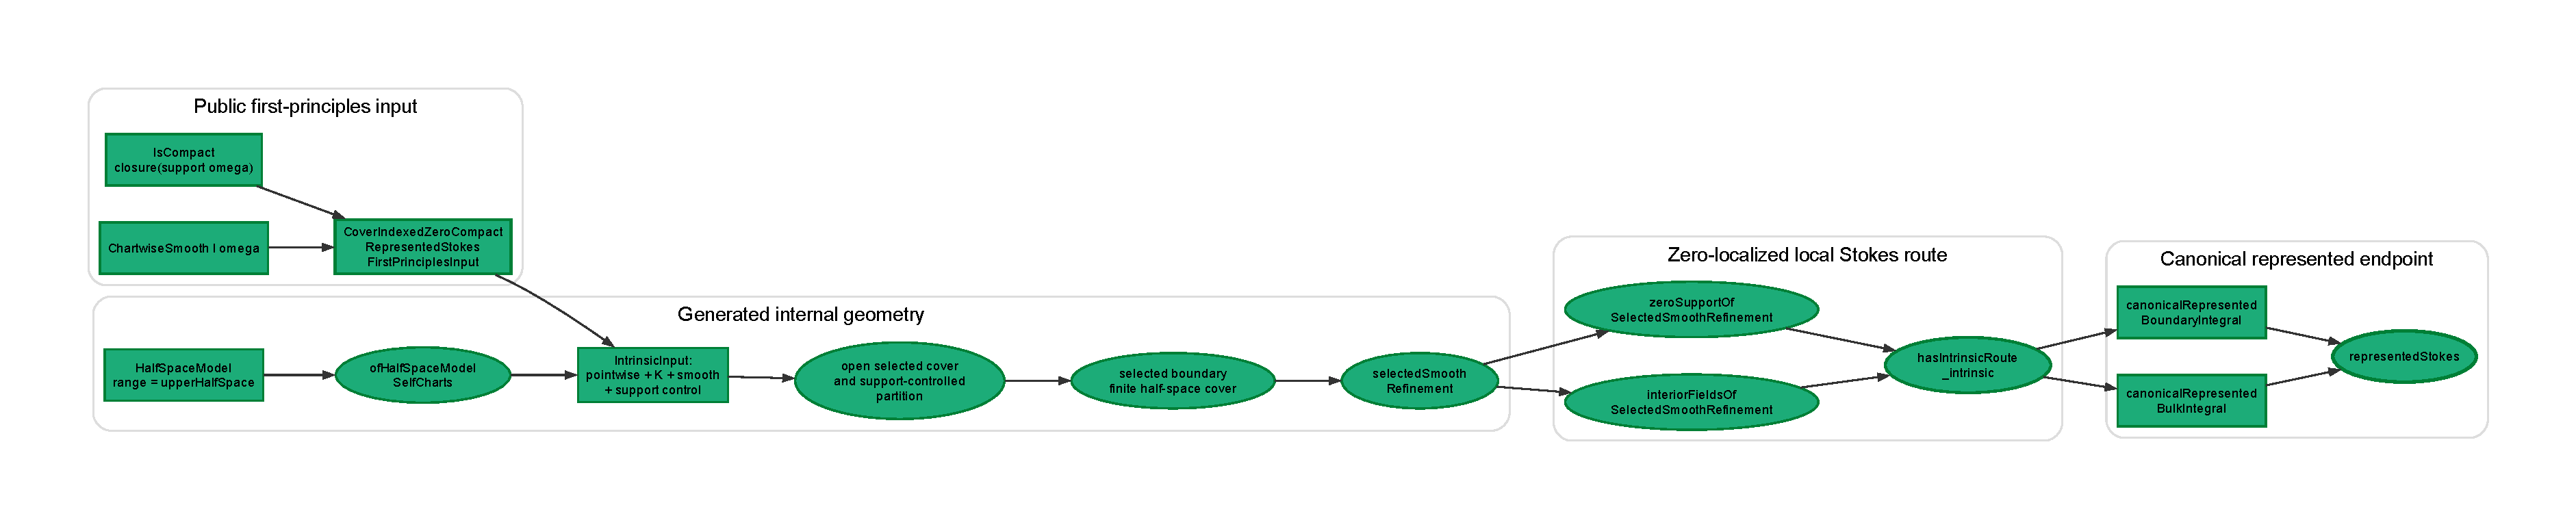
\includegraphics[width=0.94\textwidth]{figures/stokes-first-principles-graph.pdf}
  \caption{The first-principles route.  The public hypotheses generate the
  compact carrier, selected cover, support-controlled partition, smooth
  refinement, zero-localized support, local fields, and represented endpoints.
  In this and subsequent dependency figures, light-green rectangular nodes
  denote definitions or constructed data, while dark-green oval nodes denote
  theorem-level statements or derived equalities.}
  \label{fig:first-principles-route}
\end{figure}

\subsection{A useful invariant}

A recurring invariant in the development is the following:
\begin{quote}
Every local summand must carry enough support information to kill the faces
that are not part of the manifold boundary.
\end{quote}
Many intermediate certificate fields existed because this invariant had not
yet been derived from earlier data.  The final first-principles route proves
the invariant from compact support, selected open support control, and
zero-localized chart representatives.  This is the mathematical reason the
public API can be small.

\section{Formalization Obstacles as Mathematical Lemmas}
\label{sec:obstacles}

The development repeatedly encountered situations where a sentence that is
acceptable in a paper proof was not a well-formed theorem in Lean.  The useful
lesson is not that Lean is fussy.  Rather, the formalization identifies the
mathematical lemma that the sentence was abbreviating.  This section collects
five such obstacles.  They are the main reason the final theorem is stronger
than a certificate-consuming assembly theorem: each obstacle was eventually
turned into a constructor or theorem generated from compact support,
chartwise smoothness, and half-space geometry.

\begin{table}[t]
\centering
\scriptsize
\setlength{\tabcolsep}{3pt}
\begin{tabular}{p{0.19\textwidth}p{0.25\textwidth}p{0.24\textwidth}p{0.15\textwidth}}
\hline
Paper phrase & Ill-shaped Lean theorem & Corrected theorem/API & Role in Stokes \\
\hline
``smooth on the boundary box'' &
ambient smoothness on an open neighborhood of a closed box touching
\(x_0=0\) &
interior Stokes fields and open-interior/closed-box regularity &
legal boundary local Stokes \\

``the chart representative is supported in the box'' &
support of the totalized chart representative &
zero-localized representative and selected zero-support theorem &
support theorem for the correct representative \\

``the artificial faces vanish'' &
face integrals are zero by informal inspection &
face-coefficient support predicate and artificial-face remainder theorems &
removes all non-boundary box faces \\

``choose finitely many charts'' &
an arbitrary finite cover disconnected from partition support &
open shrinks, selected finite covers, and support-controlled partitions &
turns compact support into usable local data \\

``sum the local identities'' &
local sums and endpoint definitions use different finite indices &
generated represented endpoints over the same refined pieces &
global represented equality \\
\hline
\end{tabular}
\caption{Five paper-level phrases and the precise theorem shapes needed in
Lean.  The final first-principles theorem is small because the corrected
theorems are generated internally rather than exposed as public hypotheses.}
\label{tab:obstacle-map}
\end{table}

\Cref{tab:obstacle-map} is the organizing principle for this section.  Each
row is an instance of the same pattern.  The informal phrase is not false in
ordinary mathematical practice; it is a compressed reference to a more precise
lemma.  A certificate-consuming formalization can stop by asking the user to
provide that lemma.  The contribution of the final route is that the lemma is
proved from the preceding data and no longer appears as a theorem-facing
field.

\subsection{Boundary smoothness is not ambient closed-box smoothness}

The informal local proof near a boundary point often says that a coordinate
representative is smooth on a box.  If the model is a half-space, the word
``box'' hides a choice.  The closed coordinate box may touch the boundary
face \(x_0=0\).  Requiring an ambient open neighborhood of the closed box
inside the chart target is then too strong: it asks for Euclidean data across
the boundary, where the boundary chart is not intended to provide it.

The corrected mathematical lemma separates the roles of the box:
\begin{itemize}
  \item differentiability for the bulk term is needed on the open interior
  \(\prod_i(a_i,b_i)\);
  \item continuity and integrability are needed on the closed box and its
  faces;
  \item the lower normal face \(x_0=0\) is allowed to lie on the model
  boundary.
\end{itemize}
The Lean record \code{HalfSpaceBoxInteriorStokesFields} is exactly this
separation.  It is not a bureaucratic certificate; it is the local theorem
shape that avoids an invalid boundary-chart smoothness hypothesis.

The corrected theorem is not weaker; it is better aligned with the analysis.
It asks for differentiability exactly where the bulk derivative is evaluated
and for closed-box regularity exactly where the face integrals and
measure-theoretic bridges need it.  This is the difference between assuming a
Euclidean extension across the boundary and proving a half-space theorem.

\subsection{Support in a chart is not support of a total function}

The phrase ``the chart representative is supported in the box'' normally means
that the representative is supported in the box where the chart expression is
meaningful.  Lean functions are total, so the ordinary representative has
values outside the meaningful chart region.  If a theorem quantifies over the
ordinary support of that total function, it may be asking for facts about
values introduced only to make the function total.

The corrected lemma changes the representative.  This is stronger than adding
an auxiliary hypothesis to the old theorem.  The old theorem speaks about a
total function whose off-source values are artifacts of totalization; the new
theorem speaks about the local representative intended by the proof.  The
development defines a zero-localized representative which agrees with the
ordinary representative on the chart source and is zero outside.  The support
theorem is then a genuine topological statement:
\[
  \tsupp(\operatorname{ZeroRep}_{x,x}(\rho\omega))
  \subseteq Q(a,b).
\]
The Lean theorem
\code{zeroSupportOfSelectedSmoothRefinement} proves this statement for the
actual coefficients generated by the selected smooth refinement.

This is one of the main places where the formalization discovers a better
mathematical interface.  Asking the user for a support assumption on
\code{transitionPullbackInChart} would have hidden the problem.  Proving
\code{zeroSupportOfSelectedSmoothRefinement} removes the assumption by proving
that the generated representative has the support property that the informal
proof silently uses.

The theorem therefore has two parts that must travel together.  First, the
zero-localized representative agrees with the ordinary representative on the
source where the local integral is evaluated.  Second, it has global support
properties because it is zero outside the source.  Without the agreement
theorem the proof would be about the wrong local form; without the support
theorem artificial-face cancellation would still be a public assumption.

\subsection{Artificial faces vanish by support, not by notation}

When Stokes is applied on a coordinate box, every face of the box appears.  In
a boundary chart only the lower normal face is the manifold boundary.  The
other faces are artifacts of the localization.  A paper proof may say that
they vanish because the support is inside the box.  Lean requires the exact
disjointness statement for each face coefficient and each artificial face.

The corrected lemma has the following structure:
\[
  \tsupp(\alpha)\subseteq Q(a,b)
  \Longrightarrow
  \text{every artificial face integral of }\alpha\text{ is }0.
\]
This is implemented through the face-support API in the half-space layer.  The
global proof does not assume artificial-face cancellation; it derives it from
the zero-localized support theorem for each refined local representative.

The important point is that the support statement is made for face
coefficients, not only for the form as an abstract object.  The box theorem
integrates coefficients on coordinate faces.  The formalization proves that
evaluating the form on a fixed face frame does not enlarge topological
support, then uses the half-space support region to show that the artificial
face set is disjoint from those coefficient supports.

\subsection{Compactness is a construction principle}

Compact support is not merely a hypothesis that allows one to write a finite
sum.  The proof uses it to construct the finite index type, the selected
charts, the open shrinks, the partition coefficients, and the boundary
refinement.  If any of these choices is made independently, later support and
endpoint reconstruction statements can fail to line up.

The corrected lemma is a compactness-to-data theorem: compactness of \(K\)
together with pointwise chart-box neighborhoods produces a finite selected
cover with a support-controlled partition.
The selected cover remembers both the open sets used for the partition and the
closed or half-space boxes used for support.  This dual memory is what lets the
local support facts feed into half-space Stokes.

Thus compactness is used to generate an indexed object with invariants, not
only to prove existence of finitely many open sets.  The finite selected data
must remember enough information for three later consumers: the partition of
unity, the half-space local theorem, and the endpoint summation.

\subsection{Represented endpoints are finite coordinate theorems}

The last hidden step is endpoint reconstruction.  Once each local piece
satisfies Stokes, the proof still has to show that the finite sum of local
bulk terms is the generated represented bulk endpoint, and similarly for the
boundary terms.  This is not a definition-free conclusion: the local pieces
are sigma-indexed by boundary chart and refined box data.

The corrected theorem keeps the endpoint generated from the same finite data
used by the local proof.  This prevents a common mismatch: proving local
equalities over one index family and defining the global endpoint over a
slightly different one.  In the final route, the represented endpoints are
canonical because they are induced by the selected finite route itself.

This is why the represented endpoint layer is a mathematical layer rather
than a naming layer.  The endpoint is not chosen after the local proof; it is
the finite sum whose index family is shared by the cover, the refinement, the
zero-support theorem, and the local Stokes theorem.

\subsection{Summary of the compression}

Each obstacle has the same final form:
\[
  \text{informal paper step}
  \quad\leadsto\quad
  \text{precise generated Lean theorem}.
\]
The final first-principles API is small because these generated theorems
replace the large certificates that earlier routes exposed.  This is the
central mathematical engineering pattern of the project.

\section{Half-Space Local Stokes}
\label{sec:halfspace}

The boundary case is the first place where the formal proof diverges sharply
from an ordinary Euclidean box proof.  A boundary chart has image in a
half-space, not in all of \(\R^{n+1}\).  A local box may touch the boundary
face \(x_0=0\).  The correct local theorem therefore has to see the half-space
geometry, as in classical treatments of manifolds with boundary and
differential forms
\cite{warner1983foundations,abraham1988manifolds,lang1995differential,lee2013smooth}.

\subsection{What the paper proof omits}

In the paper proof, after choosing a boundary chart one often writes a local
coordinate box and applies Stokes.  The intended picture is clear: the lower
normal face is the actual boundary of the manifold, while the other faces are
introduced by the coordinate box and should not contribute if the localized
form is supported away from them.  In a proof assistant, this picture becomes
a family of statements:
\begin{itemize}
  \item the lower normal face is the face with coordinate \(x_0=a_0=0\);
  \item its sign agrees with the outward-normal-first boundary convention;
  \item the upper normal face and the tangential faces are artificial;
  \item the artificial face integrals vanish under a topological support
  condition;
  \item the local analytic assumptions are valid for a box that may touch the
  half-space boundary.
\end{itemize}

The last point is especially important.  It is tempting to require smoothness
on an ambient open neighborhood of the closed box.  That requirement is
natural for interior boxes, but it is not the right boundary hypothesis.  If
the box touches \(x_0=0\), there need not be a chart-target open set in the
ambient Euclidean space containing the closed box on both sides of the
boundary.  The bulk derivative is needed on the open box interior; the boundary
faces need continuity and integrability data.  The formal theorem separates
these assumptions instead of smuggling in an invalid ambient-open condition.

The false theorem shape is therefore:
\[
  \text{closed half-space box }[a,b]\subset U,\quad
  U\text{ ambient open},\quad U\subseteq\text{chart target}.
\]
For a boundary box with \(a_0=0\), this asks the chart target to contain
Euclidean points with negative normal coordinate near the lower face.  That is
not part of the half-space chart.  The correct statement replaces this single
ambient-open condition by separate obligations: open-interior differentiability
for the bulk term, closed-box coefficient regularity for face integrals, and
support control for artificial faces.

\subsection{The half-space primitives}

The half-space layer defines the model set, boundary inclusion, boundary
tangent frame, outward normal, and sign convention.  The relevant names include
\code{upperHalfSpace}, \code{boundaryInclusion},
\code{outwardFirstBoundaryFrame}, and \code{halfSpaceBoundarySign}.
The theorem
\[
\code{halfSpaceBoundarySign_eq_outwardFirstBoundaryOrientationSign}
\]
aligns the coordinate lower-face sign with the outward-first convention used
for the boundary.  Without this bridge, the local lower-face term would remain
a cube face term rather than the represented boundary contribution.

The support box is encoded by \code{halfSpaceSupportBox}.  It is the portion of
the coordinate box that is relevant for the half-space theorem.  The formal
support condition used by local Stokes is expressed through
\[
\code{boxFaceCoeffTSupportInHalfSpaceBox}.
\]
This condition is later obtained from the zero-localized support theorem for
the selected smooth refinement.

Geometrically, \code{halfSpaceSupportBox} is asymmetric.  In the normal
coordinate it allows contact with the lower face \(x_0=0\), because that is
the true boundary.  In the upper normal direction and in all tangential face
directions it is strict, because those faces are artificial.  This is why the
support theorem can both retain the boundary contribution and remove the rest
of the cube boundary.

\begin{theorem}[Half-space compact-support local Stokes]
\label{thm:halfspace-local}
Let \(\alpha\) be an \(n\)-form-valued coordinate representative on
\(\R^{n+1}\), and let \(a\le b\) be box corners with \(a_0=0\).  Suppose the
interior Stokes fields for \((\alpha,a,b)\) are available and the topological
support of \(\alpha\) is contained in the corresponding half-space support box.
Then
\[
  \operatorname{Bulk}_{a,b}(\alpha)
  =
  \operatorname{sgn}_{\partial\HH}\,
  \operatorname{Boundary}_{a,b}^{x_0=0}(\alpha).
\]
In Lean this is the theorem
\code{halfSpaceLocalStokes_compactSupport_of_interiorFields}.
\end{theorem}

This theorem is the local mathematical engine used by the global route.  The
left-hand side is the coordinate bulk integral of the exterior derivative
coefficient.  The right-hand side is not an arbitrary selected face: it is the
lower normal face, transported through the half-space boundary sign.

\subsection{Artificial faces}

The local Euclidean box theorem produces all faces of the box.  For a boundary
chart, only the lower normal face corresponds to the boundary of the manifold.
The remaining terms are collected in
\[
\code{halfSpaceLocalBoundaryRemainder}.
\]
The main cancellation theorem has the schematic form
\[
  \tsupp(\alpha)\subseteq Q(a,b)
  \quad\Longrightarrow\quad
  R_{a,b}(\alpha)=0.
\]
In Lean this is represented by the chain:
\begin{lstlisting}[language=Lean]
boxRemainingFormFaceTerms_eq_zero_of_tsupport_subset_halfSpaceSupportBox
halfSpaceLocalBoundaryRemainder_eq_zero_of_tsupport_subset_halfSpaceSupportBox
\end{lstlisting}
These theorems are where the informal phrase ``the support misses the
artificial boundary'' becomes a checkable proof.  They also explain why the
global theorem needs topological support control, not merely pointwise
ordinary support information.

The proof has a simple mathematical shape.  Euclidean box Stokes first writes
the bulk integral as the sum of all signed face integrals.  The half-space
boundary API identifies the lower normal face with the true boundary term.
For every other face, support containment in the half-space support box gives
disjointness between the face coefficient support and that face, so the
corresponding face integral is zero.  The remaining equality is exactly
\cref{thm:halfspace-local}.

\subsection{Proof sketch of the local theorem}

The local half-space theorem is obtained by factoring the usual box theorem
through three comparison steps.

\paragraph{Step 1: ordinary box Stokes.}
For a coordinate \(n\)-form \(\alpha\) on \(\R^{n+1}\), the Euclidean box
theorem expresses the integral of the coordinate exterior derivative over
\([a,b]\) as a signed sum over all coordinate faces.  This is the analytic
part of the proof closest to standard treatments of integration and geometric
measure theory
\cite{munkres1991analysis,rudin1987real,federer1969geometric,evans1992measure}.
In the Lean development, this is the part delegated to the box-Stokes infrastructure.  The
\code{HalfSpaceBoxInteriorStokesFields} record stores exactly the hypotheses
that this theorem consumes: continuity of signed coefficients on the closed
box, differentiability on the open box away from a countable exceptional set,
integrability of the divergence term, and the equality between the exterior
derivative coefficient and the coordinate divergence integral.

\paragraph{Step 2: identify the lower normal face.}
Because \(a_0=0\), the lower face in the normal coordinate is the model
boundary of the half-space.  The boundary integral layer proves that the
coordinate lower-face term is the half-space boundary form integral, multiplied
by the sign prescribed by the outward-first convention.  This is the content
of the lower-face and \code{halfSpaceBoundarySign} bridge lemmas.

\paragraph{Step 3: erase artificial faces.}
All remaining faces are introduced by the coordinate box.  The support box is
chosen so that a form whose topological support is contained in it has zero
face coefficient on those artificial faces.  Hence the remainder sum is zero.
This is where the global zero-support theorem is consumed by the local layer.

The result is a local theorem whose hypotheses match what boundary charts can
actually provide.  It does not require a closed box to have an ambient open
neighborhood across the boundary.

\begin{center}
\small
\begin{tabular}{p{0.28\textwidth}p{0.34\textwidth}p{0.24\textwidth}}
\hline
Local ingredient & Why it is needed & Lean location \\
\hline
open-interior differentiability & identifies the bulk derivative on the box
interior & open-interior fields \\
closed-box continuity and integrability & makes the box and face integrals
legal & interior Stokes fields \\
lower normal face sign & turns the cube face into the true boundary term &
boundary-sign lemmas \\
topological support in the half-space support region & removes every
artificial face & face-support predicate \\
\hline
\end{tabular}
\end{center}

\subsection{Interior fields}

The record
\begin{lstlisting}[language=Lean]
structure HalfSpaceBoxInteriorStokesFields
    (omega : (Fin (n + 1) -> Real) ->
      (Fin (n + 1) -> Real) [/\^Fin n]->L[Real] Real)
    (a b : Fin (n + 1) -> Real) where
  le : a <= b
  lower_zero : a 0 = 0
  exceptional : Set (Fin (n + 1) -> Real)
  exceptional_countable : exceptional.Countable
  continuous_signedCoeff : ...
  hasFDerivAt_signedCoeff : ...
  integrable_divergence : ...
  bulk_eq_boxIntegral : ...
\end{lstlisting}
packages exactly what the half-space local theorem needs from the Euclidean
box theorem.  The exceptional set and differentiability fields match the
interface of the underlying box-divergence theorem.  The field
\code{bulk_eq_boxIntegral} bridges the mathlib exterior derivative integrand
and the coordinate divergence integrand used by the box theorem.

This record is the point where the formalization makes a mathematical
distinction that a paper proof can blur.  There is no single phrase
``smooth on the box'' that supplies all of these facts in the boundary case.
Some facts live on the open interior, some on the closed box, and some are
a.e. comparisons between two integrands.  Bundling them into
\code{HalfSpaceBoxInteriorStokesFields} gives the exact contract consumed by
local Stokes, after which later constructors prove the fields automatically
for the selected refined representatives.

The theorem
\begin{lstlisting}[language=Lean]
theorem halfSpaceLocalStokes_compactSupport_of_interiorFields
\end{lstlisting}
then turns these fields plus artificial-face support control into the local
compact-support half-space Stokes identity.  The version
\[
\code{HalfSpaceBoxInteriorStokesFields.withRemainder}
\]
keeps the artificial-face remainder visible, while
\[
\code{HalfSpaceBoxInteriorStokesFields.compactSupport}
\]
uses support containment to remove it.

\subsection{From chartwise smoothness to local fields}

The first-principles theorem does not ask the user for
\code{HalfSpaceBoxInteriorStokesFields}.  Those fields are generated by:
\begin{lstlisting}[language=Lean]
CoverIndexedZeroCompactRepresentedStokesIntrinsicInput.
  interiorFieldsOfSelectedSmoothRefinement
\end{lstlisting}
The constructor uses chartwise smoothness of the original form, smoothness of
the selected refined coefficients, and the fact that the selected closed boxes
lie in the self chart transition source.  It constructs open-interior
smoothness fields and then applies
\[
\code{HalfSpaceBoxInteriorStokesFields.ofOpenInteriorSmoothness}.
\]

The mathematical point is that closed-box regularity is proved for the actual
localized coordinate form on the selected box, while bulk differentiability is
used on the open box interior.  This prevents the global theorem from
depending on a false boundary-chart ambient-open hypothesis.

This split is also important for degenerate boxes.  Some coordinate intervals
may collapse during finite refinement.  In such cases, the closed-box
regularity and integrability statements remain meaningful, while the open
interior may be empty or lower dimensional.  The local fields isolate the
measure-theoretic bridge needed by the box theorem so that degenerate and
nondegenerate cases can be handled uniformly by the surrounding constructors.

\begin{figure}[t]
  \centering
  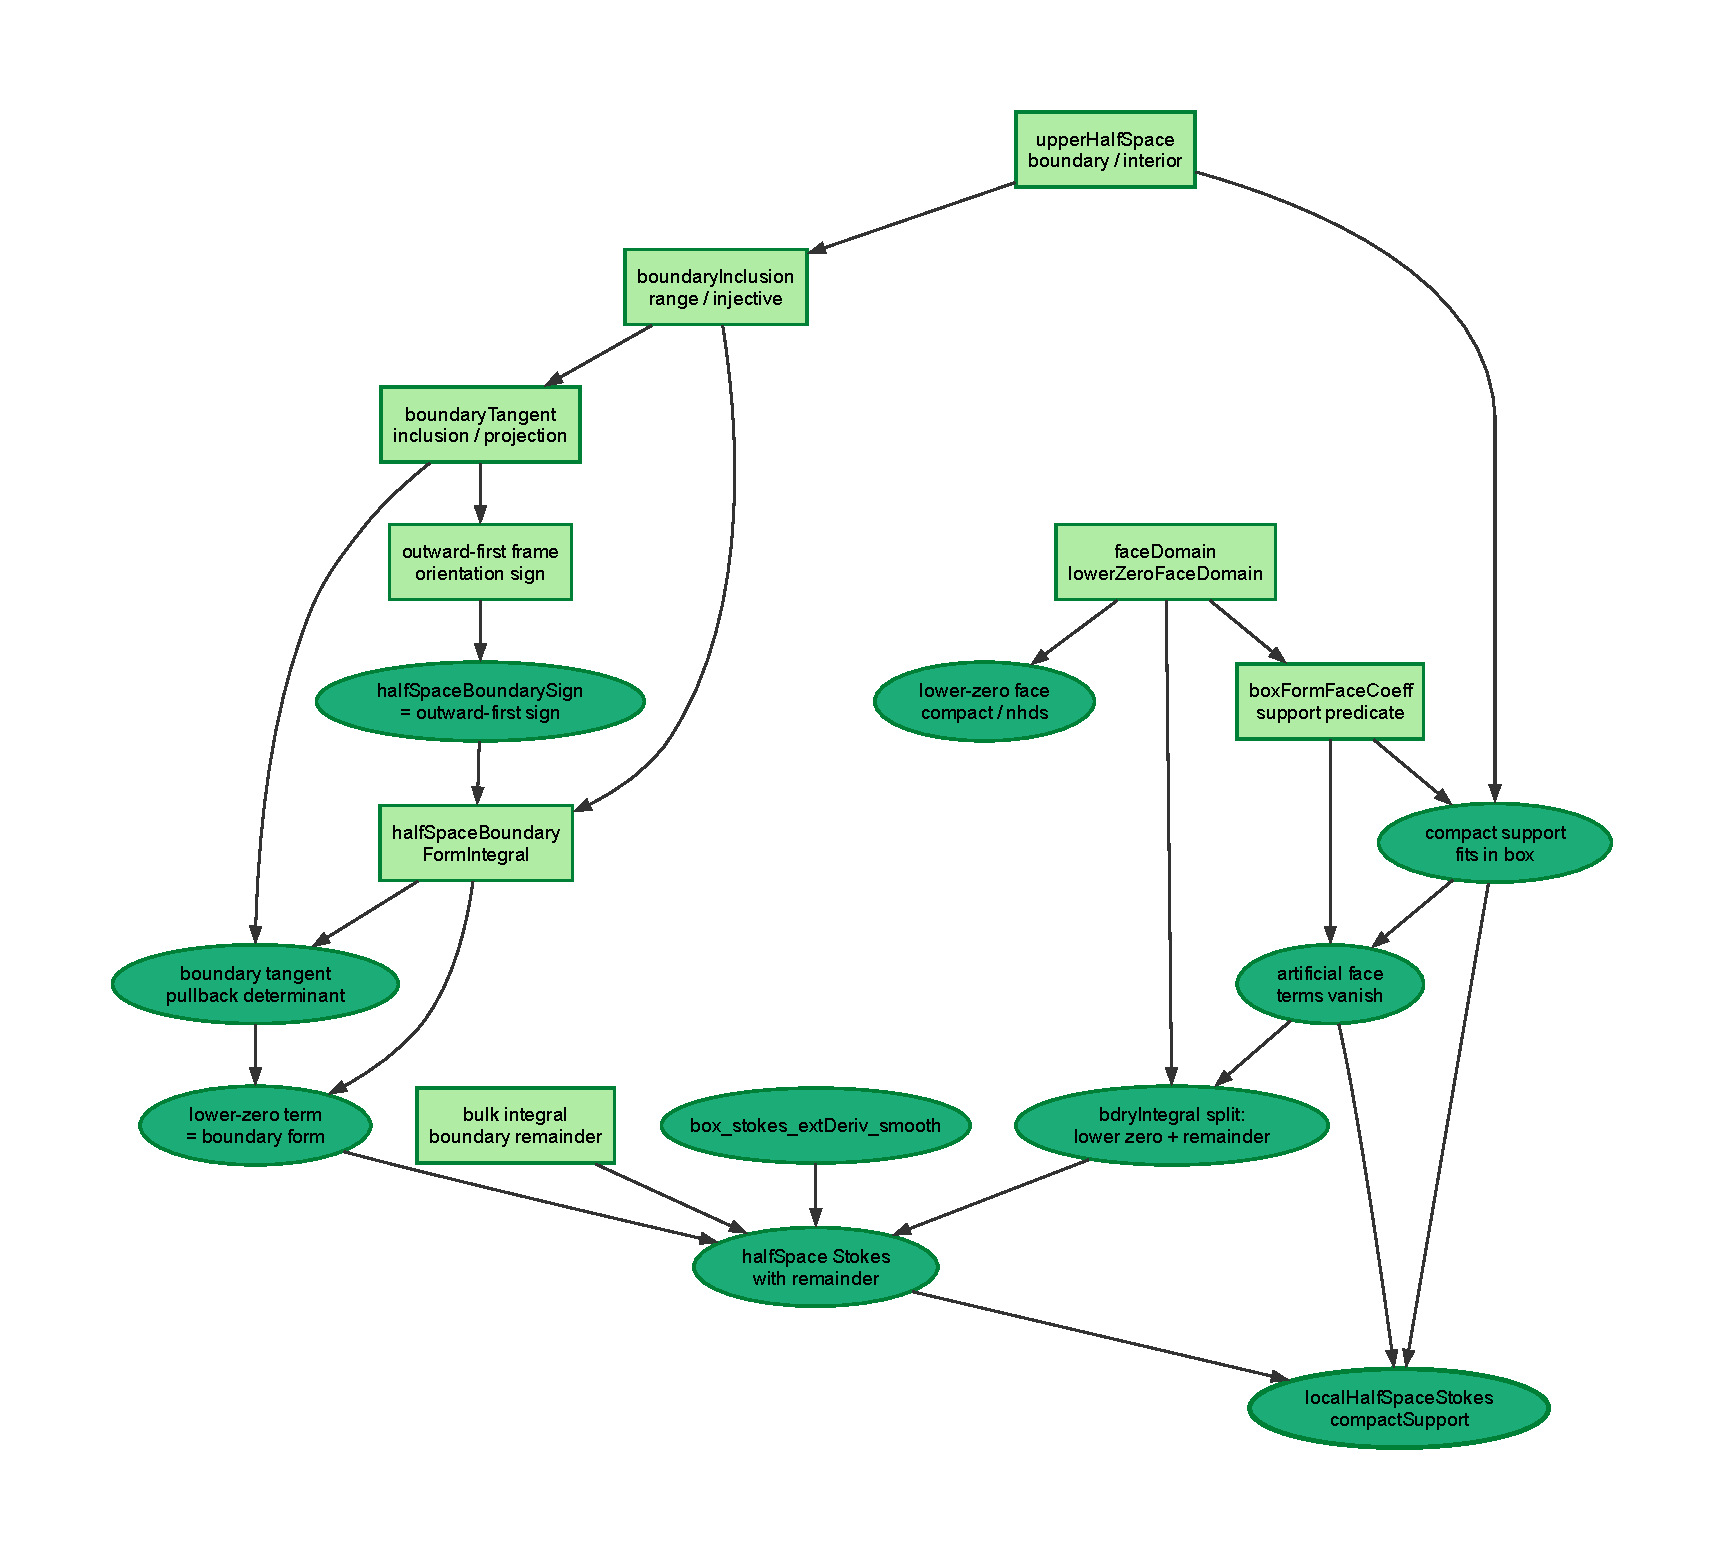
\includegraphics[width=0.86\textwidth]{figures/stokes-halfspace-graph.pdf}
  \caption{The half-space layer separates the true lower boundary face from
  artificial coordinate faces, and separates open-interior differentiability
  from closed-box face regularity.  Light-green rectangular nodes denote
  definitions or constructed data; dark-green oval nodes denote theorem-level
  statements or derived equalities.}
  \label{fig:halfspace-layer}
\end{figure}

\subsection{Why this layer is substantive}

It would be possible to state a global theorem assuming a local Stokes theorem
for every selected box.  The artifact does more: it builds the local theorem
from the half-space box infrastructure and then connects it to the selected
refined representatives.  This is why the final theorem can hide local Stokes
fields.  The local half-space content is not absent from the public API; it is
proved and generated internally.

\section{Support and Zero-Localization}
\label{sec:zero-localization}

The most deceptive obstacle in the formalization is support.  Mathematicians
habitually speak about a chart representative only where the chart is defined.
Lean does not.  A chart representative is a total function, and its support is
a global statement about that total function.  The central discovery of this
part of the development is that the problem cannot be solved by asking for a
stronger support hypothesis on the same representative.  The representative
itself has to be changed.

\subsection{The false support theorem}

Suppose \(\rho\) is a partition coefficient and \(\omega\) is a form.  A paper
proof may say that the coordinate representative of \(\rho\omega\) is
supported in a coordinate box \(Q\).  In Lean, the corresponding ordinary
representative is
\[
\code{ManifoldForm.transitionPullbackInChart}.
\]
It has a value at every coordinate point.  Outside the chart source, target, or
overlap, those values are artifacts of totalization.  Thus a theorem of the
form
\[
\tsupp(\code{transitionPullbackInChart}(\rho\omega)) \subseteq Q
\]
may be too strong or simply unrelated to the informal argument.  It asks Lean
to control the chart representative even at points where the coordinate
description should not be considered part of the local proof.

This problem explains several early certificate fields in the development.  It
is easy to request a support assumption from the user.  It is harder, and more
mathematically faithful, to prove the right theorem from compact support and
partition support control.  The right theorem is not about the unrestricted
total representative.

One can view the issue as a small counterexample pattern.  Suppose a chart
expression is mathematically intended only on a set \(U\), but Lean represents
it by some total function \(f : E \to V\).  Even if \(f\) is perfectly
controlled on \(U\), its values on \(E\setminus U\) may enlarge
\(\operatorname{support}(f)\).  A theorem about \(\operatorname{support}(f)\)
is therefore not the same as a theorem about the local representative on
\(U\).  The zero-localized representative replaces \(f\) by
\[
  y\mapsto
  \begin{cases}
    f(y), & y\in U,\\
    0, & y\notin U,
  \end{cases}
\]
so that global support again expresses the intended local support.  This is a
change of object, not a notational convenience.

\begin{remark}[The false support theorem]
The tempting theorem is:
\[
  \tsupp(\code{transitionPullbackInChart}(\rho\omega))\subseteq Q.
\]
The formalization treats this as the wrong target.  The values of
\code{transitionPullbackInChart} outside the transition source are present
because Lean functions are total, not because the local coordinate proof has
mathematical content there.  Strengthening the hypotheses to control those
values would make the final theorem depend on an artifact of representation.
The corrected target is the same inclusion for the zero-localized
representative, together with an agreement theorem on the transition source.
\end{remark}

\subsection{Zero outside the chart domain}

The project introduces a zero-localized representative:
\[
\code{ManifoldForm.transitionPullbackInChartZero}.
\]
It agrees with \code{transitionPullbackInChart} on the relevant chart source
and is zero outside.  The basic API proves:
\begin{itemize}
  \item support is contained in the source;
  \item support is contained in the target;
  \item support is contained in the overlap;
  \item the zero representative agrees with the ordinary representative on
  the chart source.
\end{itemize}
The core names are:
\begin{lstlisting}[language=Lean]
transitionPullbackInChartZero_support_subset_source
transitionPullbackInChartZero_support_subset_target
transitionPullbackInChartZero_support_subset_overlap
transitionPullbackInChartZero_eqOn_transitionPullbackInChart
\end{lstlisting}

This changes the meaning of support control.  Instead of proving that a
totalized chart function behaves well outside its mathematical domain, the
proof makes the representative zero there by definition and proves support
properties for the resulting function.  The point is not simply that zero
extension is available; it is that the zero extension is the formal object
corresponding to the informal phrase ``the local chart representative''.

The equality theorem is as important as the support theorem.  The zero
representative must agree with the ordinary representative on the region where
local integration is performed; otherwise the theorem would prove Stokes for a
different object.  This is why the API includes both support inclusions and
agreement theorems such as
\code{transitionPullbackInChartZero_eqOn_transitionPullbackInChart}.

The zero-localization API therefore has a three-part mathematical shape:
\[
\begin{array}{ll}
\text{definition} & \text{make the off-source representative zero},\\
\text{support theorem} & \text{prove source, target, and overlap support},\\
\text{agreement theorem} & \text{recover the ordinary chart expression on the
source}.
\end{array}
\]
All three are needed.  The definition alone would give a different
representative; the agreement theorem makes it harmless for integration on
the selected box; the support theorem makes artificial-face cancellation
available.

\subsection{Localized forms}

The global proof uses localized forms \(\rho\omega\).  Zero-localization has to
interact with localization.  The theorem
\[
\code{ManifoldForm.transitionPullbackInChartZero_localizedForm}
\]
rewrites the zero-localized representative of a localized form as the product
of the coefficient representative and the zero-localized representative of the
base form.  From this, the project proves support inclusions such as
\[
\code{transitionPullbackInChartZero_localizedForm_tsupport_subset_coefficient}
\]
and
\[
\code{transitionPullbackInChartZero_localizedForm_tsupport_subset_form}.
\]

The decisive bridge is:
\begin{lstlisting}[language=Lean,basicstyle=\ttfamily\scriptsize]
transitionPullbackInChartZero_localizedForm_tsupport_subset_halfSpaceSupportBox_of_support_subset_K
\end{lstlisting}
It formalizes the following argument:
\[
\begin{array}{c}
\supp(\omega)\subseteq K,\\
\tsupp(\rho)\cap K\text{ is controlled by the selected chart box},\\
\text{the coordinate image of the active carrier is controlled},\\
\hline
\tsupp(\text{zero-localized representative of }\rho\omega)
  \subseteq \text{selected half-space support box}.
\end{array}
\]
This is the support theorem the half-space local Stokes layer needs.

\begin{lemma}[Zero-localized support bridge]
\label{lem:zero-support}
Let \(K\) be a compact carrier containing \(\supp(\omega)\).  Let \(\rho\) be a
localization coefficient whose topological support on \(K\) is contained in a
coordinate carrier, and suppose that the coordinate image of that carrier is
contained in a half-space support box \(Q(a,b)\).  Then the zero-localized chart
representative of \(\rho\omega\) has topological support contained in
\(Q(a,b)\).
\end{lemma}

This lemma is the formal replacement for the informal statement that
``\(\rho\omega\) is supported in the selected box.''  The latter statement is
ambiguous in a total-function setting; the former is a precise theorem about
the representative actually used by the local Stokes theorem.

At the level of Lean proof dependencies, the bridge decomposes as follows:
\[
\begin{array}{c}
\tsupp(\operatorname{ZeroRep}(\rho\omega))
  \subseteq
  \tsupp(\rho\text{ in chart}),\\[2mm]
\tsupp(\operatorname{ZeroRep}(\rho\omega))
  \subseteq
  \tsupp(\operatorname{ZeroRep}(\omega)),\\[2mm]
\tsupp(\operatorname{ZeroRep}(\omega))
  \subseteq \operatorname{chartImage}(K),\\[2mm]
\tsupp(\rho\text{ in chart})\cap \operatorname{chartImage}(K)
  \subseteq Q(a,b),\\[2mm]
\hline
\tsupp(\operatorname{ZeroRep}(\rho\omega))\subseteq Q(a,b).
\end{array}
\]
The first two inclusions are product-support facts.  The third is the global
compact-support input transported through the zero representative.  The last
line is the selected-refinement support control.  Their combination is exactly
the support bridge displayed above.

There are two support operations in the proof.  Ordinary support is algebraic:
it records where a function is nonzero.  Topological support is the closure of
ordinary support and is the right object for face-disjointness and vanishing
integrals.  The development therefore does not stop at ordinary nonzero-set
control.  The final local Stokes input is a \(\tsupp\)-level inclusion into a
selected half-space support region.  That region is designed to allow contact
with the true boundary face \(x_0=0\) while strictly avoiding the artificial
faces of the coordinate box.

\subsection{Selected smooth refinement}

The final route applies the preceding bridge to the canonical smooth
refinement selected by the first-principles theorem.  The theorem is:
\begin{lstlisting}[language=Lean]
CoverIndexedZeroCompactRepresentedStokesIntrinsicInput.
  zeroSupportOfSelectedSmoothRefinement
\end{lstlisting}
states that for every selected boundary index \(i\) and active refined
half-space piece \(q\), the topological support of the zero-localized
representative of the refined localized form is contained in the selected
half-space support box:
\[
\tsupp
  \left(
    \operatorname{ZeroRep}
    \bigl(\rho_{i,q}\omega\bigr)
  \right)
  \subseteq
  \code{halfSpaceSupportBox}(a_{i,q},b_{i,q}).
\]
Here \(\rho_{i,q}\) is not a user-supplied coefficient.  It is the coefficient
generated by the selected smooth refinement.

This point is crucial for the first-principles theorem.  If \(\rho_{i,q}\)
were arbitrary, the zero-support theorem would be false.  It is true because
\(\rho_{i,q}\) is built from the selected boundary partition and the selected
smooth subpartition, both of which carry support-control data from the
compactness construction.

The proof uses a two-stage localization identity.  The refined coefficient is
the product of the selected boundary partition coefficient and the smooth
subpartition coefficient.  The proof rewrites
\[
  \rho_{i,q}\omega
  =
  \theta_{i,q}(\rho_i\omega)
\]
and then uses the support of \(\rho_i\omega\) to place the form in the
boundary active carrier, while the support of \(\theta_{i,q}\) places the
coordinate representative inside the refined half-space box.

\begin{proof}[Proof idea for the selected theorem]
The proof first shows that the boundary-localized form \(\rho_i\omega\) is
supported in the boundary active carrier.  This uses the algebraic fact that
support of a localized form is contained in the support of the coefficient and
in the support of the original form, together with
\(\supp(\omega)\subseteq K\).  Next, the smooth subpartition coefficient
\(\theta_{i,q}\) is known, on that active carrier, to be supported inside the
selected refined half-space box.  The zero-localized product formula transfers
these two support facts to the chart representative.  The proof is carried out
at the level of topological support for the coefficient and the zero base
representative, using the product-support inclusions
\[
  \tsupp(fg)\subseteq\tsupp(f),
  \qquad
  \tsupp(fg)\subseteq\tsupp(g).
\]
Thus the theorem delivered to the half-space layer is already the required
\(\tsupp\)-inclusion; it is not a fragile ordinary-support statement later
patched by hand.
\end{proof}

\subsection{Ordinary support versus topological support}

Another formal distinction is ordinary support versus topological support.
Many algebraic arguments first show that if a function is nonzero at a point,
then that point lies in a desired set.  But artificial-face vanishing is a
closed-support statement.  The theorem must control
\[
  \tsupp(f)=\overline{\{x\mid f(x)\ne0\}}.
\]
In the half-space box proof the target support region is not a naive closed
box.  The set \(\code{halfSpaceSupportBox}(a,b)\) allows the support to meet
the true lower normal face, but uses strict inequalities in the directions
corresponding to artificial faces.  This is exactly the geometry needed by the
face-cancellation theorem: it proves that the artificial face set is disjoint
from the topological support.  Consequently the proof is organized to produce
\(\tsupp\)-statements directly for the localized coefficients and
zero-localized representatives.

Closed-set upgrades still appear in the surrounding support infrastructure in
the familiar form
\[
  \operatorname{support}(f)\subseteq C,\quad C\text{ closed}
  \quad\Longrightarrow\quad
  \tsupp(f)\subseteq C.
\]
But the final half-space input is more specific: it is a topological-support
inclusion into a region chosen so that artificial faces are avoided and the
true boundary face is retained.  This is why the support theorem is not merely
``the coefficient is zero on the face.''  It is a coordinated package of
zero-extension, product support, compact carrier support, and half-space box
geometry.

\subsection{Contribution to the global theorem}

Zero-localized support is the bridge between compact finite data and local
Stokes.  The support-controlled partition and smooth refinement produce
coefficient support information.  Zero-localization turns it into support
information for the coordinate form representative.  The half-space layer then
uses that support information to remove artificial faces.  Without this bridge,
the final theorem would have to expose an unnatural support assumption for
ordinary total chart representatives.  With it, the first-principles theorem
requires no such field.

\section{Compact Support to Finite Data}
\label{sec:compact-finite-data}

Compact support is the theorem's main global hypothesis.  In the proof, it is
not used as a passive assumption.  It is the mechanism that turns pointwise
chart geometry into a finite coordinate calculation.  This is the constructive
content of the compact-support proof found in classical differential-form
treatments, where compactness, partitions of unity, and local coordinate
Stokes are used together
\cite{munkres1991analysis,bott1982differential,morita2001geometry,lee2013smooth}.

\subsection{The compact carrier}

The first-principles theorem fixes the carrier
\[
  K = \overline{\supp(\omega)}.
\]
This choice is made by the definition
\[
\code{CoverIndexedZeroCompactRepresentedStokesFirstPrinciplesInput.supportCarrier}.
\]
The public compactness field is
\[
\code{IsCompact (closure (ManifoldForm.support I omega))}.
\]
The support inclusion needed by the intrinsic route is then simply
\(\supp(\omega)\subseteq \overline{\supp(\omega)}\), discharged internally by
\code{subset_closure}.

This design matters because it removes an otherwise arbitrary carrier from the
public theorem.  Earlier routes allowed a user to choose a compact set \(K\)
and prove \(\supp(\omega)\subseteq K\).  That is mathematically reasonable, but
the first-principles form expresses the standard compact-support hypothesis
directly: the closure of the support is compact.

This choice also fixes the direction of later support proofs.  Every
localized summand is ultimately controlled by showing that its nonzero points
come from nonzero points of \(\omega\), hence lie in \(K\).  The theorem never
needs the user to guess a larger carrier with additional geometric properties.
All geometry is generated from the canonical carrier.

This is a small but important interface decision.  A theorem with an arbitrary
compact carrier \(K\) is useful internally, but it leaves the user responsible
for choosing a carrier that will later interact well with charts, partitions,
and support control.  The first-principles theorem fixes the canonical choice
and proves the required inclusion automatically.  In this way the compactness
hypothesis is stated exactly as compact support of the form.

\subsection{Pointwise chart boxes from the half-space model}

The intrinsic route requires pointwise chart-box data on \(K\).  The
first-principles theorem does not expose that data.  It is generated from the
half-space model using self charts:
\begin{lstlisting}[language=Lean]
PointwiseCompactSupportChartBoxData.ofHalfSpaceModelSelfCharts
\end{lstlisting}
The background class
\[
\code{HalfSpaceModel}
\]
records that the model range is the upper half-space.  From this, the
development proves that self-chart coordinates land in the half-space and can
be separated into boundary and interior cases.

At an interior coordinate point, one chooses a box contained in the positive
normal region.  At a boundary coordinate point, one chooses a half-space box
whose lower normal coordinate is zero.  The constructor proves the
neighborhood and box-containment facts required by the selected-cover layer.
Thus the pointwise geometry is no longer a user-facing certificate.

\subsection{Open shrinks}

Closed or half-closed chart boxes are not the right objects for constructing a
partition of unity.  The formal proof therefore chooses auxiliary open shrinks
inside the pointwise chart boxes.  This is encoded in
\code{PointwiseCompactSupportChartBoxData.OpenShrink} and:
\begin{lstlisting}[language=Lean]
PointwiseCompactSupportChartBoxData.selectedOpenCoverOfPointwise
\end{lstlisting}
The selected open cover remembers both the open set used for partition
construction and the assigned closed or half-space chart box used later for
support containment.

The proof pattern is:
\begin{quote}
pointwise chart-box neighborhood \(\Rightarrow\) open shrink inside the chart
box \(\Rightarrow\) finite selected open cover by compactness.
\end{quote}
This is one of the places where Lean forces a useful distinction.  A
neighborhood fact is not itself a globally selected open cover with finite
index type and assigned box data.  The formalization constructs that object.

The full construction chain is:
\[
\begin{array}{c}
\text{pointwise chart-box neighborhood at each }x\in K\\
\Downarrow\\
\text{open shrink }U_x\text{ with }x\in U_x\subseteq\text{assigned box}\\
\Downarrow\\
\text{finite selected open cover by compactness}\\
\Downarrow\\
\text{support-controlled partition subordinate to the selected cover}\\
\Downarrow\\
\text{boundary active carriers and finite half-space refinements}.
\end{array}
\]
Every arrow carries data used later.  The selected open set is needed for the
partition theorem; the assigned box is needed for support containment; the
finite index type is needed for endpoint reconstruction.

\begin{lemma}[Compactness-to-finite-selection]
\label{lem:compact-finite-selection}
Pointwise chart-box neighborhood data on a compact carrier \(K\) determines a
finite selected chart-box cover of \(K\), after choosing open shrinks inside
the pointwise boxes.  Moreover, the selected cover remembers both the open
sets used to build partitions and the assigned coordinate boxes used for later
support containment.
\end{lemma}

This is mathematically the finite-subcover step, but the formal statement is
stronger than a bare finite cover: it preserves enough bookkeeping to connect
partition support, chart boxes, and later half-space refinement.

The finite selection has three pieces of information that must travel
together.  First, it has a finite index type.  Second, each index remembers the
chosen chart and whether it is treated as an interior or boundary chart.  Third,
each index remembers an assigned box that contains the support portion of the
eventual partition coefficient.  Omitting any one of these pieces would force a
later theorem to reintroduce a manual compatibility hypothesis.

This is the first major certificate-elimination step in the global proof.
Earlier routes accepted selected covers and openness data as public inputs.
The final route proves that they are consequences of pointwise chart-box
neighborhoods and compactness, and the first-principles route generates the
pointwise data from the half-space model.

\subsection{Support-controlled partitions}

The partition used by the theorem is not merely a family summing to one.  It is
a support-controlled selected partition:
\[
\code{OpenSupportControlledSelectedPartition}.
\]
The key guarantee is that the topological support of a partition coefficient,
intersected with the compact carrier, lies inside the assigned selected open
set and then inside the assigned chart box:
\begin{lstlisting}[language=Lean]
openSupportControlledSelectedPartition_tsupport_inter_subset_assigned
\end{lstlisting}

This statement is later used twice.  First, it proves that the first boundary
localization \(\rho_i\omega\) is supported in the boundary active carrier.
Second, after smooth refinement, it contributes to the proof that each refined
localized zero representative is supported inside its half-space support box.
Without support control at the partition stage, artificial-face vanishing would
have to be assumed later.

The support-controlled partition is stronger than the usual partition of unity
existence theorem in exactly the way Stokes needs
\cite{guillemin1974differential,hirsch1976differential,warner1983foundations,tu2011introduction}.
It is not enough that
\(\sum_i\rho_i=1\) on \(K\).  We need
\[
  \tsupp(\rho_i)\cap K \subseteq U_i
\]
for the selected open shrink \(U_i\), and then \(U_i\) must itself lie inside
the assigned chart box.  This is the route by which compactness and partitions
eventually become a statement about artificial coordinate faces.

\subsection{Boundary active carriers}

For a selected boundary index \(i\), the boundary active carrier is the part of
\(K\) where the boundary partition coefficient is active.  Its coordinate
image is the set that must be covered by half-space boxes.  In the intrinsic
route, the selected boundary boxes themselves provide the coordinate ambient
sets:
\begin{lstlisting}[language=Lean]
SupportControlledSelectedPartition.finiteHalfSpaceCoverOfSelectedBoundaryBoxes
\end{lstlisting}
This avoids the older public fields for boundary ambient sets and collar-prism
certificates.  The theorem now derives the finite half-space cover from the
selected boundary box geometry generated earlier.

\subsection{Smooth refinement}

The finite half-space cover still has to be converted into smooth refined
coefficients.  This is handled by
\begin{lstlisting}[language=Lean]
CoverIndexedZeroCompactRepresentedStokesIntrinsicInput.selectedSmoothRefinement
\end{lstlisting}
The surrounding API proves:
\begin{lstlisting}[language=Lean]
selectedSmoothRefinementAmbientOpen
isOpen_selectedSmoothRefinementAmbientOpen
boundaryActiveCarrier_subset_iUnion_selectedSmoothRefinementAmbientOpen
selectedSmoothRefinementAmbientOpen_subset_boundaryChartBox
\end{lstlisting}

The smooth refinement introduces a sigma-indexed family of pieces.  A boundary
index \(i\) may have many active refined boxes \(q\).  The theorem
\[
\code{selectedSmoothRefinement_boundaryPieces}
\]
connects the refinement's boundary pieces with the selected finite half-space
cover.  This connection is used by the endpoint route to ensure that the same
pieces are used for support, local Stokes, and finite-sum reconstruction.

The refined coefficient has the form
\[
  \rho_{i,q}(x)=\rho_i(x)\,\psi_{i,q}(x),
\]
where \(\rho_i\) is the selected boundary partition coefficient and
\(\psi_{i,q}\) is the smooth subpartition coefficient subordinate to the
refined half-space box.  The identity
\[
  \sum_{q\in Q_i}\rho_{i,q}(x)=\rho_i(x)
\]
on the relevant carrier is the algebraic reason the refined local sums
reconstruct the original boundary-localized contribution.

The smooth refinement is also where the endpoint index set becomes visible.
Before refinement there is one boundary coefficient \(\rho_i\) for each
selected boundary chart.  After refinement the local half-space theorem is
applied to the family \(\rho_{i,q}\), indexed by a boundary chart and a
selected refined box.  The endpoint layer must use precisely this same
sigma-indexed family; otherwise local Stokes would be proved for one finite
sum and the represented endpoint would be defined over another.

\begin{figure}[t]
  \centering
  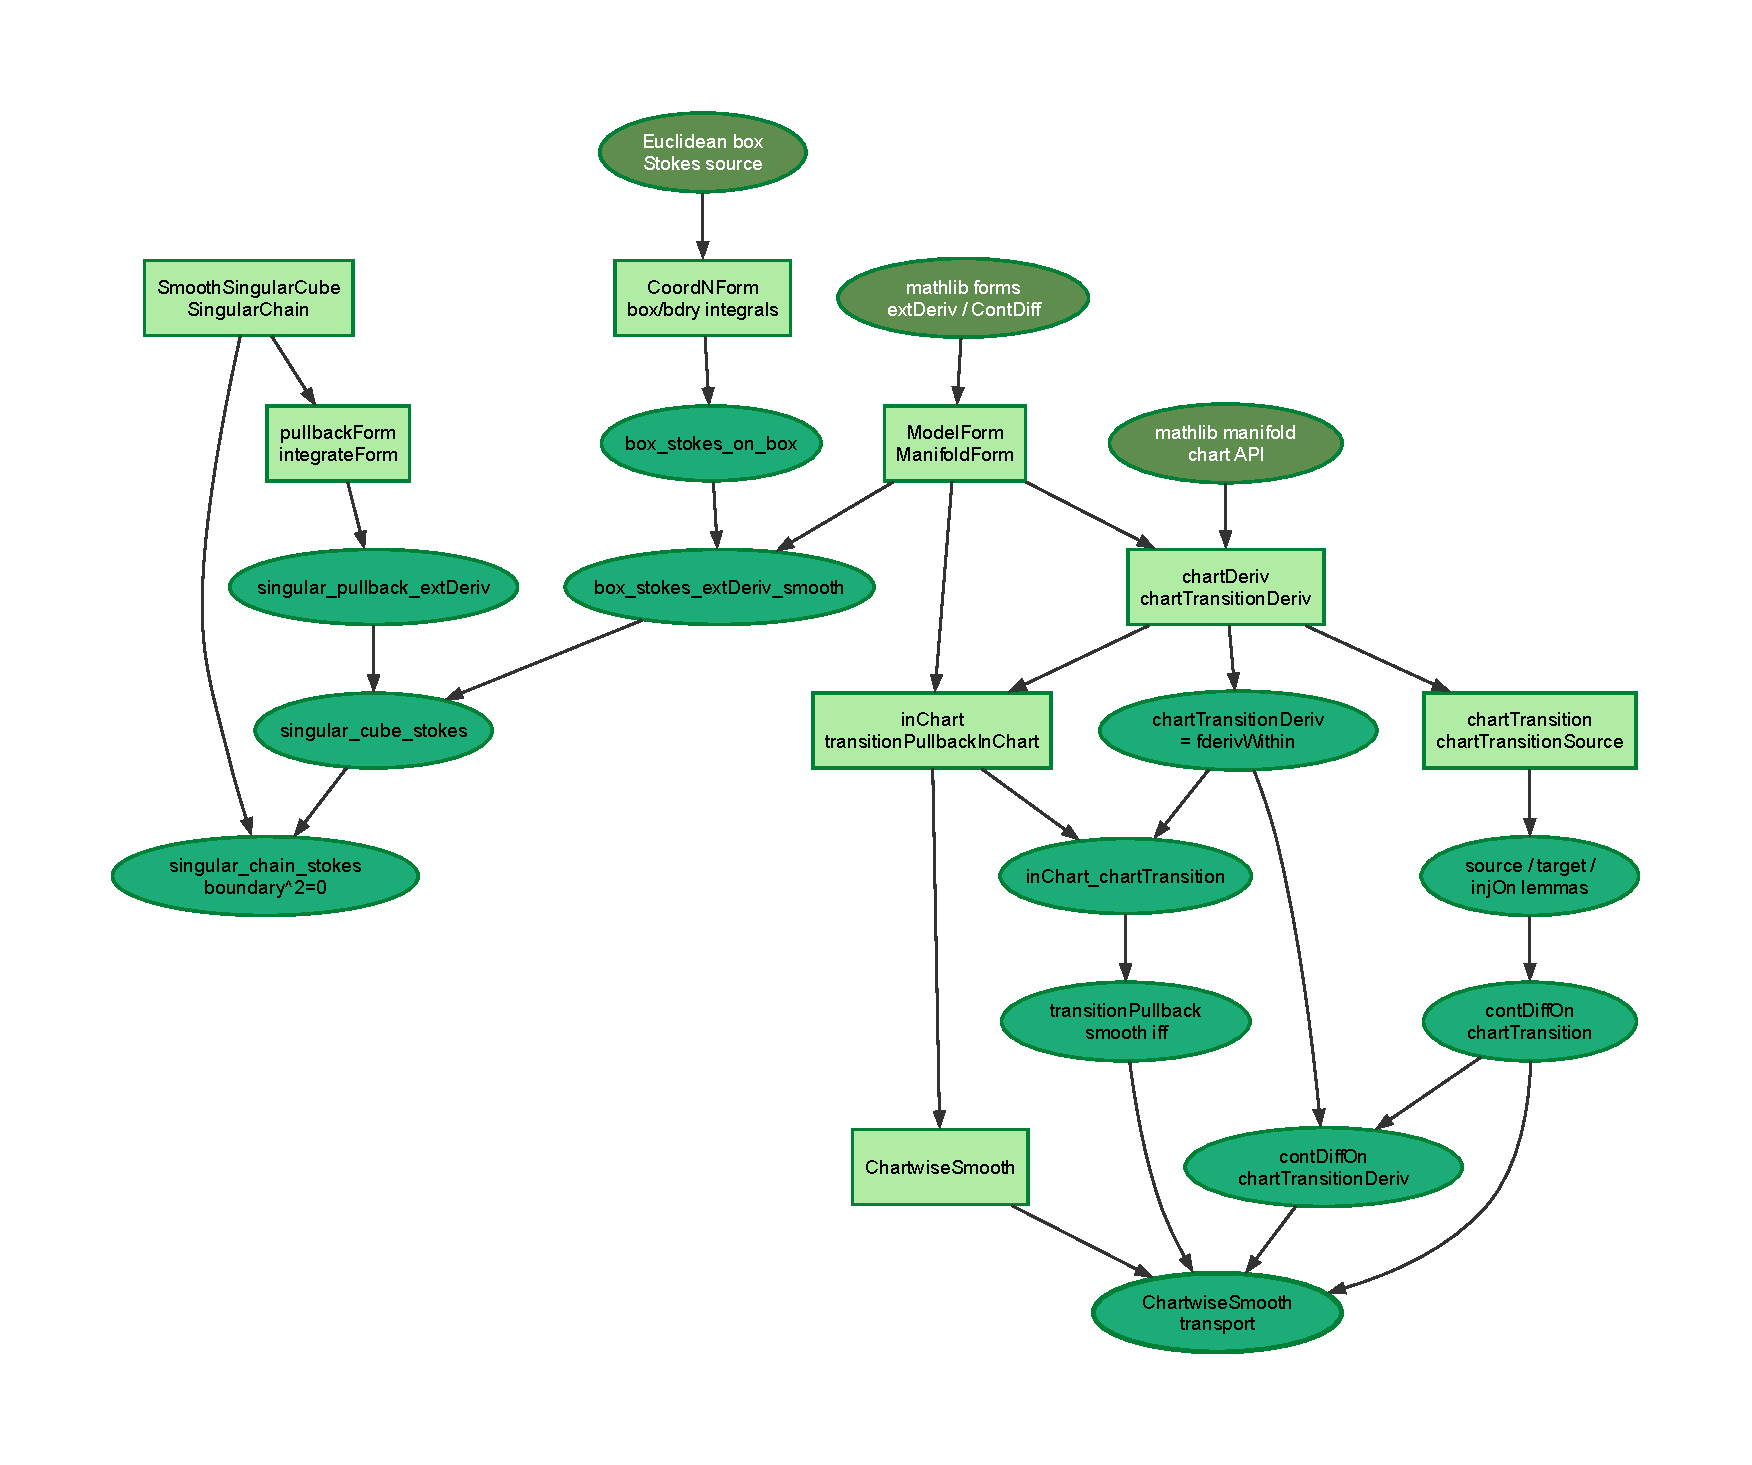
\includegraphics[width=0.92\textwidth]{figures/stokes-core-graph.pdf}
  \caption{The compactness and refinement core: compact support gives a finite
  selected cover; support-controlled partitions and smooth refinements prepare
  the local half-space Stokes data.  Light-green rectangular nodes denote
  definitions or constructed data; dark-green oval nodes denote theorem-level
  statements or derived equalities.}
  \label{fig:core-graph}
\end{figure}

\subsection{Why finite data is not bookkeeping}

The finite selected data is the skeleton of the represented theorem.  It
determines the index types of the endpoint sums, the coefficients of the
localized forms, the boxes on which local Stokes is applied, and the support
facts used to remove artificial faces.  A mismatch between any two of these
finite structures would make the final reconstruction theorem false or
unusable.

The first-principles theorem hides the finite data from users because Lean
constructs it internally.  It does not make the data irrelevant.  The data is
the mechanism by which compact support becomes a finite coordinate Stokes
proof.

In this sense, compactness is not a side condition of Stokes but a generator
of the proof route.  It selects the charts, fixes the partition coefficients,
determines which boundary carriers are active, and supplies the index sets for
the represented endpoints.  The final theorem can have a small input because
this generated finite data is coherent by construction.

\begin{remark}
The support-controlled partition is the reason compactness can be used once,
near the beginning of the proof, rather than reintroduced as local hypotheses
for every box.  Once the finite selected data is built, all later support facts
are consequences of the selected construction.
\end{remark}

\section{Endpoint Reconstruction}
\label{sec:endpoint-reconstruction}

After each refined local piece satisfies half-space Stokes, the proof still has
to reconstruct a global represented equality.  This section explains why the
endpoint layer is a mathematical component of the formalization rather than a
renaming of local terms.

\subsection{Nested finite sums}

The selected boundary refinement is indexed in two stages.  There is a finite
set of boundary chart indices \(i\), and for each \(i\) a finite set of active
refined pieces \(q\).  The local theorem gives
\[
  \code{localBulkTerm}(i,q)=\code{localBoundaryTerm}(i,q)
\]
for every active pair.  Summing gives
\[
  \sum_i\sum_{q\in Q_i}\code{localBulkTerm}(i,q)
  =
  \sum_i\sum_{q\in Q_i}\code{localBoundaryTerm}(i,q).
\]

In Lean, this is not merely an algebraic observation.  The finite sets
\(Q_i\) must be definitionally or propositionally connected with the selected
half-space cover, the smooth refinement, and the local Stokes data.  The
endpoint structure is designed to keep those indices aligned.

The guiding invariant is that the same active pair \((i,q)\) performs three
roles at once: it chooses the half-space box, chooses the refined coefficient,
and appears in the endpoint sum.
If any of these are separated, the proof acquires adapter fields whose only
purpose is to prove that two finite descriptions are the same.  The localized
endpoint layer avoids this by generating the endpoint from the refined pieces
that already carry the local Stokes data.

\begin{lemma}[Finite endpoint summation]
\label{lem:endpoint-summation}
Given a localized refined endpoint with finite boundary pieces \(Q_i\), if
\[
  B_{i,q}=C_{i,q}
\]
for every active refined piece \(q\in Q_i\), then the generated represented
endpoints satisfy
\[
  \sum_i\sum_{q\in Q_i} B_{i,q}
  =
  \sum_i\sum_{q\in Q_i} C_{i,q}.
\]
The Lean endpoint layer instantiates \(B_{i,q}\) as
\code{localBulkTerm i q} and \(C_{i,q}\) as
\code{localBoundaryTerm i q}.
\end{lemma}

The lemma looks elementary, but its Lean version is valuable because it fixes
the finite index family once and for all.  The same membership proof
\(q\in Q_i\) is used to access the box corners, the coefficient, the local
form, the zero-support theorem, and the local Stokes fields.  This prevents
the proof from silently changing finite sums when moving between local and
global layers.

The proof itself has three algebraic steps.  First, it rewrites the generated
bulk endpoint as the nested sum of the local bulk terms.  Second, it rewrites
each local bulk term using the per-box Stokes equality.  Third, it folds the
resulting nested sum back into the generated boundary endpoint.  In a paper
proof these are often collapsed into the phrase ``summing over the cover.''
In Lean they are separate because every sum carries its index type and
membership conditions.

\subsection{Localized refined partitions}

The core endpoint structure is
\[
\code{CoverIndexedBoundaryLocalizedRefinedPartition}.
\]
It stores the refined boundary pieces and the generated local bulk and
boundary terms.  Its definitions
\[
\code{generatedRepresentedBulkIntegral}
\]
and
\[
\code{generatedRepresentedBoundaryIntegral}
\]
are the represented endpoints at this layer.  The theorem
\[
\code{representedStokes_of_localStokes}
\]
turns a finite family of local equalities into equality of these generated
endpoints.

The zero-localized route refines this through
\[
\code{CoverIndexedBoundaryLocalizedRefinedPartition.ZeroLocalStokesData}.
\]
This record stores the specific local data needed to apply the half-space
local theorem to zero-localized representatives.  It includes source and
target charts, local forms, box corners, zero-support information, and the
local terms whose equality will be summed.

The localized refined partition is intentionally smaller than the older global
endpoint certificates.  It does not attempt to encode every possible future
native integral comparison.  It records the data needed to state and prove the
represented finite-sum equality.  This makes it a stable target: future
comparison theorems can map from this generated endpoint to native integrals
without changing the local Stokes proof.

This design also prevents the represented theorem from depending on a future
choice of native manifold integration API.  The endpoint structure fixes the
finite coordinate equality now; a later native bridge can prove that this
finite coordinate quantity agrees with a chosen global integral definition.

\subsection{From zero local Stokes data to endpoints}

The theorem
\[
\code{ZeroLocalStokesData.localStokes_of_interiorFields}
\]
builds the per-box local Stokes equality from interior fields and zero support.
Then
\[
\code{boundaryHalfSpaceBulkSum_eq_trueBoundarySum_of_zeroLocalStokesData}
\]
proves the nested finite-sum equality.  Finally,
\[
\code{representedStokes_of_zeroLocalStokesData}
\]
reconstructs equality of the generated represented endpoints.

\begin{theorem}[Zero-localized endpoint reconstruction]
For the localized refined partition generated by the intrinsic route, the
combination of zero support and half-space interior fields implies equality of
the generated represented bulk and boundary endpoints.  In Lean this is the
role of:
\begin{lstlisting}[language=Lean]
CoverIndexedBoundaryLocalizedRefinedPartition.
  representedStokes_of_zeroLocalStokesData
\end{lstlisting}
\end{theorem}

The first-principles route uses the constructor
\[
\code{hasIntrinsicRoute_of_selectedSmoothRefinement}
\]
to assemble the endpoint, zero-localized local data, boundary piece equality,
zero support, and interior fields into an intrinsic certificate.  Once the
canonical selected smooth refinement supplies the last two ingredients, the
intrinsic route has a canonical endpoint equality.

The role of this constructor is precisely to avoid exposing an endpoint
adapter to the final user.  It proves that the endpoint, local Stokes data,
zero-support theorem, and regularity fields are all generated from the same
selected smooth refinement.  Thus the endpoint equality is not imported from
outside the proof; it is assembled from the local Stokes theorem over the
canonical finite route.

\subsection{Canonical endpoints at the top level}

The intrinsic input defines
\[
\code{canonicalRepresentedBulkIntegral}
\quad\text{and}\quad
\code{canonicalRepresentedBoundaryIntegral}
\]
by choosing the route generated from the canonical selected smooth refinement:
\[
\code{hasIntrinsicRoute_intrinsic}.
\]
The first-principles input then projects these endpoints through its generated
intrinsic input.  Thus the top-level definitions are not external names.  They
are the endpoint definitions induced by the canonical finite selected route.

\subsection{Why reconstruction matters}

Endpoint reconstruction is where the represented theorem becomes global.  The
half-space local theorem knows only about one coordinate box.  Zero-localized
support knows only how to kill artificial faces for one refined representative.
Compactness and refinement know how to generate finitely many such pieces.
The endpoint layer proves that all of these local facts assemble into one
equality between the two canonical represented quantities associated with the
input form.

This is also the layer that makes the represented-to-native future work
well-posed.  A future theorem comparing represented endpoints with native
manifold integrals can target
\[
\code{canonicalRepresentedBulkIntegral}
\quad\text{and}\quad
\code{canonicalRepresentedBoundaryIntegral}
\]
directly.  It does not need to rediscover the local proof route.

There is an important conceptual payoff here.  The proof does not define a
global endpoint first and then ask local lemmas to match it.  Instead, the
endpoint is generated from the same local pieces used by the proof.  This
removes a common source of mismatch in large formalizations: the local theorem,
the summation theorem, and the final theorem all quantify over the same finite
piece data.

This is why the word canonical is warranted in the represented theorem.  It
does not mean independent of every possible choice of partition or chart cover;
that would be the native comparison problem.  It means canonical relative to
the generated first-principles route: once the input form is fixed, the route
constructs a selected finite proof object, and the endpoints are the finite
sums determined by that object.

\subsection{What remains for native integrals}

Endpoint reconstruction stops at the finite coordinate equality.  To obtain a
future native theorem, one must prove two comparison results.  The bulk
comparison identifies the represented bulk sum with the chosen definition of
\(\int_M\dd\omega\).  The boundary comparison identifies the represented
lower-face sum with the chosen definition of \(\int_{\partial M}\omega\) under
the global boundary orientation.  These comparisons are logically downstream
from the represented theorem: they should not be mixed into the proof that the
finite coordinate endpoints are equal.

\section{Main Lean Theorem}
\label{sec:main-theorem}

The preferred public theorem is located in
\[
\code{Stokes/Global/CoverIndexedZeroCompactRepresentedStokesFirstPrinciples.lean}.
\]
It is re-exported through the slim public cover-indexed import.  This section
records the theorem shape and the internal route.

\subsection{Ambient Lean context}

The theorem is stated for a space \(M\) charted over a model \(H\), with model
with corners
\[
  I : \code{ModelWithCorners Real (Fin (n + 1) -> Real) H}.
\]
The surrounding Lean context includes the usual manifold and topological
assumptions used by the route, expressed using the typeclass and structure
mechanisms of Lean and mathlib
\cite{demoura2015lean,demoura2021lean4,baanen2022instance,mathlib2020}:
\[
\code{IsManifold I top M},\quad
\code{T2Space M},\quad
\code{SigmaCompactSpace M},
\]
finite dimensionality of the coordinate model, and the half-space model
assumption
\[
\code{HalfSpaceModel I}.
\]
The half-space model is a background geometric assumption: it tells Lean that
the model range is the upper half-space and supports the automatic construction
of pointwise boundary and interior chart boxes.

\subsection{First-principles input}

The public input structure is:
\begin{lstlisting}[language=Lean]
structure CoverIndexedZeroCompactRepresentedStokesFirstPrinciplesInput
    (I : ModelWithCorners Real (Fin (n + 1) -> Real) H)
    (omega : ManifoldForm I M n) where
  chartwiseSmooth : ManifoldForm.ChartwiseSmooth I omega
  compactSupport : IsCompact (closure (ManifoldForm.support I omega))
\end{lstlisting}
There is no public selected cover, no partition field, no boundary ambient
field, no collar-prism certificate, no local Stokes field, and no endpoint
adapter.  These objects are generated internally.

The compact carrier is:
\begin{lstlisting}[language=Lean]
def supportCarrier : Set M :=
  closure (ManifoldForm.support I omega)
\end{lstlisting}
The intrinsic input is built by:
\begin{lstlisting}[language=Lean]
def intrinsicInput :
    CoverIndexedZeroCompactRepresentedStokesIntrinsicInput
      (I := I) (omega := omega) supportCarrier where
  pointwise :=
    PointwiseCompactSupportChartBoxData.ofHalfSpaceModelSelfCharts
      (I := I) supportCarrier
  hK := X.compactSupport
  chartwiseSmooth := X.chartwiseSmooth
  support_subset_K := subset_closure
\end{lstlisting}
This is the first major compression: the four-field intrinsic theorem is
generated from the two-field first-principles theorem.

\subsection{Canonical represented endpoints}

The top-level endpoints are:
\begin{lstlisting}[language=Lean]
def canonicalRepresentedBulkIntegral : Real :=
  (X.intrinsicInput (I := I) (omega := omega)).
    canonicalRepresentedBulkIntegral

def canonicalRepresentedBoundaryIntegral : Real :=
  (X.intrinsicInput (I := I) (omega := omega)).
    canonicalRepresentedBoundaryIntegral
\end{lstlisting}
They inherit their meaning from the intrinsic route: finite selected cover,
selected smooth refinement, zero-localized local data, half-space local
Stokes, and endpoint reconstruction.

\subsection{The theorem}

The theorem is:
\begin{lstlisting}[language=Lean]
theorem representedStokes :
    X.canonicalRepresentedBulkIntegral (I := I) (omega := omega) =
      X.canonicalRepresentedBoundaryIntegral (I := I) (omega := omega) := by
  simpa [canonicalRepresentedBulkIntegral,
    canonicalRepresentedBoundaryIntegral] using
    (X.intrinsicInput (I := I) (omega := omega)).
      representedStokes
\end{lstlisting}
The proof is short because the intrinsic theorem has already generated the
route:
\begin{lstlisting}[language=Lean]
selectedSmoothRefinement
zeroSupportOfSelectedSmoothRefinement
interiorFieldsOfSelectedSmoothRefinement
hasIntrinsicRoute_intrinsic
representedStokes
\end{lstlisting}

\subsection{Intrinsic route}

The intrinsic structure still has four mathematical fields:
\begin{lstlisting}[language=Lean]
structure CoverIndexedZeroCompactRepresentedStokesIntrinsicInput
    (K : Set M) where
  pointwise : PointwiseCompactSupportChartBoxData I K
  hK : IsCompact K
  chartwiseSmooth : ManifoldForm.ChartwiseSmooth I omega
  support_subset_K : ManifoldForm.support I omega <= K
\end{lstlisting}
It is useful as an internal theorem-facing layer.  It states the theorem with a
chosen compact carrier and pointwise chart-box data.  The first-principles
theorem hides both by choosing \(K=\overline{\supp(\omega)}\) and generating
pointwise data from the half-space model.

The intrinsic route defines the selected cover, partition, and boundary finite
cover through:
\begin{lstlisting}[language=Lean]
openSelectedCover
selectedCover
openSelectedPartition
selectedPartition
selectedBoundaryFiniteCover
\end{lstlisting}
The canonical smooth refinement is generated by
\[
\code{selectedSmoothRefinement}.
\]
The two critical automatically generated proof obligations are:
\[
\code{zeroSupportOfSelectedSmoothRefinement}
\]
and
\[
\code{interiorFieldsOfSelectedSmoothRefinement}.
\]
Together they feed into
\[
\code{hasIntrinsicRoute_intrinsic}.
\]

\begin{theorem}[First-principles represented Stokes]
\label{thm:first-principles}
In the half-space model context, chartwise smoothness of \(\omega\) and
compactness of \(\overline{\supp(\omega)}\) imply equality of the canonical
represented bulk and boundary endpoints generated by the compact-support
local-to-global route.
\end{theorem}

The proof of \cref{thm:first-principles} is not an invocation of a black-box
global theorem.  It is the composition of the following generated statements:
compactness produces selected finite data; selected finite data produces a
smooth half-space refinement; the refinement produces zero-localized support
and analytic interior fields; local half-space Stokes gives each refined
identity; and endpoint reconstruction sums those identities.

\subsection{Reading the theorem mathematically}

Mathematically, the final theorem says:

\begin{quote}
For a chartwise smooth \(n\)-form on a half-space-modeled smooth manifold, if
the closure of its support is compact, then the finite coordinate bulk endpoint
generated by the compact-support Stokes proof equals the finite coordinate
boundary endpoint generated by the same proof.
\end{quote}

This is the clean statement the development was organized to reach.  The
large amount of internal code exists so that the theorem can be stated in this
small form without making the user provide the hidden proof objects.

\section{Artifact and Scale}
\label{sec:artifact-scale}

The project is a large Lean artifact, not a short isolated formalization.  The
active \code{Stokes/} directory contains 544 Lean files and approximately
165006 Lean lines.  This scale reflects both the mathematics and the proof
engineering required to compress a certificate-heavy development into a small
public theorem.  The maintenance and interface issues are in the same family
as those discussed for large mathematical libraries such as mathlib
\cite{vandoorn2020maintaining,baanen2022instance,baanen2025growing}.

\subsection{Repository organization}

The artifact repository is available at
\url{https://github.com/evaristebernhard/Stokes} (accessed 29 May 2026).
The active Lean files live under \code{Stokes/}.  The main public route is
exported by
\[
\code{Stokes.Global.CoverIndexedFirstPrinciples}
\]
and by the slimmed cover-indexed public entry
\[
\code{Stokes.Global.CoverIndexed}.
\]
Historical routes remain available as implementation or compatibility modules,
but the default public surface is centered on the first-principles theorem.

The proof archaeology documents used to prepare this paper live under
\code{docs/formalization-log/}.  They record the mathematical bottlenecks
behind support, zero-localization, half-space boundaries, compact finite
selection, endpoint reconstruction, and API slimming.  These documents are not
part of the trusted proof base, but they are useful for explaining the
artifact.

\subsection{Public API slimming}

During development, several intermediate theorem shapes exposed internal
certificates: raw selected covers, clean inputs, natural inputs, collar routes,
endpoint adapters, image-control packages, local Stokes fields, and manual
support assumptions.  These stages were useful because they stabilized the
statement while independent local obligations were being proved.  The final
API is the result of removing those theorem-facing fields.

The first-principles theorem is therefore best viewed as a compression result,
but not in the superficial sense of putting a small facade around a large
record.  It proves that the records which earlier routes consumed are
generated by the mathematical hypotheses.  In this sense the artifact moves
from a certificate-consuming interface to a certificate-generating interface.
It does not bypass the hidden proof objects.  It constructs them internally and
then applies the intrinsic represented theorem.  This explains why a short
top-level proof can rest on a large body of Lean code.

\subsection{Route evolution}

The development history is visible in route names such as Raw, Clean, Natural,
Intrinsic, and FirstPrinciples.  These names should not be read as competing
theorems of equal status.  They record a field-elimination process.

\begin{center}
\begin{tabular}{ll}
\hline
Route style & Main theorem-facing burden \\
\hline
Raw & selected cover and low-level local data are explicit \\
Clean & several geometric certificates are packaged but still visible \\
Natural & generated data starts replacing manual endpoint fields \\
Intrinsic & pointwise chart-box data, compactness, and support control remain \\
FirstPrinciples & only chartwise smoothness and compact closed support remain \\
\hline
\end{tabular}
\end{center}

The engineering point is that intermediate routes made hidden obligations
visible.  Once an obligation could be generated from earlier mathematical
data, it moved out of the public input.  The final theorem is therefore not
another layer of ceremony; it is the accumulated result of proving that the
former certificate fields are consequences of the natural hypotheses.

\subsection{Verification gates}

The development is checked by the standard Lean build commands.  For the paper
claim, the relevant commands are:
\begin{lstlisting}
lake build Stokes
rg "\bsorry\b|\badmit\b|^\s*axiom\b" --glob "*.lean"
\end{lstlisting}
The theorem-level axiom audit is:
\begin{lstlisting}
#print axioms
  Stokes.CoverIndexedZeroCompactRepresentedStokesFirstPrinciplesInput.representedStokes
\end{lstlisting}
The expected output contains the standard Lean/mathlib axioms:
\[
\code{propext},\quad \code{Classical.choice},\quad \code{Quot.sound}.
\]

This paper rewrite does not rerun the full Lean build, because it modifies only
\code{paper/}.  The Lean names quoted in the text were checked by lightweight
repository search against the active sources.

\subsection{What scale bought}

The artifact's size bought several mathematical reductions:
\begin{itemize}
  \item ordinary total chart support assumptions were replaced by
  zero-localized support theorems;
  \item boundary-chart ambient-open assumptions were replaced by half-space
  interior and closed-box regularity fields;
  \item user-supplied finite covers and refinements were replaced by
  compactness-driven selected constructions;
  \item endpoint adapters were replaced by generated localized refined
  endpoints;
  \item theorem-facing geometric certificates were internalized behind the
  first-principles route.
\end{itemize}

These reductions are the main proof-engineering achievement of the project.
They also make the theorem usable as a stable milestone: future work can build
native integral comparison theorems against the canonical represented
endpoints rather than against a moving collection of intermediate certificates.

The zero-localized support reduction is representative of the whole pattern.
The old theorem-facing hypothesis would have asked the user to control the
support of an ordinary totalized chart representative.  The final route proves
instead that the generated zero-localized representative has the required
topological support.  This removes a bad hypothesis by replacing the object of
the theorem and then proving the comparison and support facts needed to use it.

\subsection{Artifact reading guide}

A reader who wants to audit the mathematics should start from the
first-principles theorem, then follow the intrinsic route backward: canonical
endpoint, intrinsic route certificate, selected smooth refinement, zero support,
interior fields, and half-space local Stokes.  A reader who wants to audit the
engineering should instead compare the historical route modules with the
public import surface.  The key question is not how many modules exist, but
which assumptions remain theorem-facing.  In the current preferred API, the
answer is exactly the first-principles pair: chartwise smoothness and compact
closed support.

\section{Related Work}
\label{sec:related-work}

\subsection{Lean and mathlib}

The formalization is implemented in Lean 4
\cite{demoura2015lean,demoura2021lean4,leanprover,tpil4} and builds on mathlib
\cite{mathlib2020,mathlibdocs,vandoorn2020maintaining,baanen2025growing}.  The project follows the mathlib-compatible
strategy of using existing topology, analysis, manifolds, finite-dimensional
calculus, and exterior-algebra infrastructure where possible.  The local box
Stokes layer is organized around mathlib-style divergence and differentiability
interfaces rather than a separate analytic foundation.

The theorem also exposes places where future mathlib APIs would be valuable.
In particular, the represented-to-native bridge would naturally depend on a
stable API for integrating differential forms on oriented manifolds with
boundary, together with chart-independence and boundary-orientation comparison
theorems.

\subsection{Prior Lean Stokes artifacts}

The repository treats \code{d0d1/lean-stokes-theorem} as prior work and a Lake
dependency reference \cite{leanstokes}.  That project is useful prior art for
Stokes formalization, especially around cubical or smooth-singular-cube
approaches.  Because of licensing considerations, this project uses external
developments as references rather than as copied source.  The present
contribution is different in emphasis: it formalizes a compact-support
coordinate-represented local-to-global route through chart boxes,
support-controlled partitions, half-space boundary boxes, zero-localized
representatives, and generated represented endpoints.

\subsection{Classical manifold treatments}

Classical treatments of manifolds and differential forms provide the
mathematical background for chartwise local arguments, partitions of unity,
compact support, boundary orientations, and Stokes' theorem
\cite{spivak1965calculus,munkres1991analysis,guillemin1974differential,bott1982differential,hirsch1976differential,warner1983foundations,abraham1988manifolds,lang1995differential,tu2011introduction,lee2013smooth,morita2001geometry}.
The formalization can be read as a detailed elaboration of the proof steps
that such texts compress.  The point is not that those steps are
mathematically surprising to a geometer.  The point is that their exact
dependencies become visible when the proof is checked by Lean.

This is especially visible for boundary charts.  Classical accounts freely
move between the local half-space model, the true boundary face, and the
auxiliary faces of a coordinate box.  In Lean these become separate theorems:
the lower face must be identified with the boundary contribution, the sign
must match the outward-first convention, and every artificial face must be
removed by a support theorem.

\subsection{Formalized mathematics and proof engineering}

The work also sits in a broader theorem-proving ecosystem.  Coq/Rocq,
Isabelle/HOL, and HOL Light have long provided reference points for formalized
mathematics and proof engineering
\cite{bertot2004coqart,nipkow2002isabelle,harrison2009handbook,wiedijk2006seventeen,harrison2014history}.
Within that ecosystem, formalized analysis and geometry have repeatedly
required substantial library and interface work, for example filters and
analysis in Isabelle/HOL, smooth manifolds in Isabelle/HOL, formalized Haar
measure, and the change-of-variables theorem in mathlib
\cite{holzl2013filters,immler2019smooth,vandoorn2021haar,gouezel2022change}.

Large formalizations often spend much of their effort on interfaces: finding
the right theorem boundary, replacing manual certificates by constructors, and
organizing local lemmas so that global statements have natural hypotheses.
Prominent formalization projects such as CompCert
\cite{leroy2009formal}, the formal four-color theorem
\cite{gonthier2008fourcolor}, the machine-checked odd-order theorem
\cite{gonthier2013machine}, the formal proof of the Kepler conjecture
\cite{hales2017kepler}, Schemes in Lean \cite{buzzard2022schemes},
formalized Galois theory \cite{browning2022galois}, and the Liquid Tensor
Experiment \cite{scholze2022liquid} illustrate that the
architecture of a large proof artifact is part of the contribution.  This
project is an example in differential geometry and analysis.  The intermediate
routes were not abandoned failures; they were stages in identifying which
fields were true mathematical hypotheses and which were internal proof
objects.  The first-principles theorem is the compressed result of that
interface work.

This distinction matters for evaluating formalized mathematics.  A
certificate-consuming theorem may be enough to close a proof internally, but it
does not yet present the theorem in the form a mathematician expects to use.
The present artifact treats assumption compression as part of the mathematical
work.  Covers, refinements, support facts, local regularity records, and
endpoint reconstruction are not left as user obligations once they can be
generated from compact support and chartwise smoothness.  This agrees with a
broader view of formalization as both theorem proving and mathematical
interface design \cite{avigad2018mechanization,baanen2022instance}.

The support and zero-localization layer is also an example of a common
phenomenon in formalization: a statement that is harmless on paper becomes
false or ill-shaped when all functions are total.  The solution is not merely a
technical patch.  It identifies the correct formal representative of the
informal mathematical object.

\section{Limitations and Future Work}
\label{sec:limitations}

The theorem proved by the artifact is a coordinate-represented compact-support
Stokes theorem.  This is a strong local-to-global result, but it is not the
final possible theorem about native manifold integrals.  This section states
the boundary of the claim and the natural next steps.

\subsection{Represented-to-native comparison}

The main remaining mathematical bridge is to identify the generated represented
endpoints with a chosen native integration API.  The desired comparison would
identify \code{canonicalRepresentedBulkIntegral} with \(\int_M\dd\omega\) and
\code{canonicalRepresentedBoundaryIntegral} with
\(\int_{\partial M}\omega\).
Such a bridge should prove that the finite coordinate sums generated by the
local proof are independent of the selected cover and partition and agree with
the native integral definitions.  This requires a stable target API for
integration of differential forms on oriented smooth manifolds with boundary.

The current theorem deliberately stops before this comparison.  It proves the
finite coordinate equality generated by Stokes, leaving the comparison with
native integrals as a separate theorem layer.

\subsection{Orientation and boundary APIs}

The half-space layer already proves the local sign bridge between the lower
normal face and the outward-first convention.  A full native theorem will need
to connect this local sign convention to a global boundary orientation API.
That includes transporting orientations through charts, proving compatibility
under chart changes, and connecting boundary measures or integrals with the
coordinate lower-face terms.

\subsection{Consolidation}

The repository still contains historical routes and compatibility modules.
They are valuable as development records and as local theorem sources, but the
public API should remain centered on the first-principles route.  Future
engineering work can continue to consolidate implementation modules, move
historical theorem shapes out of default imports, and keep theorem-facing
names focused on the final mathematical interface.

\subsection{Possible extensions}

Several extensions are natural:
\begin{itemize}
  \item comparison of represented endpoints with native integrals;
  \item a compact oriented smooth manifold with boundary theorem once the
  native integration bridge is in place;
  \item more systematic chart-independence lemmas for represented endpoints;
  \item upstreaming general-purpose half-space and support-localization lemmas
  to mathlib where appropriate;
  \item a shorter conference version emphasizing the artifact architecture and
  verification gates.
\end{itemize}

These are extensions of the current milestone, not repairs of it.  The present
artifact already proves the generated coordinate Stokes equality from
first-principles compact-support hypotheses.


\section*{Acknowledgements}
The author used AI-assisted programming and proof-engineering tools during the
development of the Lean artifact and the preparation of this manuscript.  All
mathematical statements, Lean theorem references, citations, and final claims
were reviewed and are the responsibility of the author.

\appendix
\section{Key Lean Statements}
\label{app:key-statements}

This appendix records simplified versions of the main Lean statements.  The
snippets omit universe parameters, typeclass context, and many implicit
arguments.  They are intended as a reader's guide to the formal theorem shapes,
not as copy-paste source.

\subsection{First-principles input and theorem}

\begin{lstlisting}[language=Lean,basicstyle=\ttfamily\footnotesize]
structure CoverIndexedZeroCompactRepresentedStokesFirstPrinciplesInput
    (I : ModelWithCorners Real (Fin (n + 1) -> Real) H)
    (omega : ManifoldForm I M n) where
  chartwiseSmooth : ManifoldForm.ChartwiseSmooth I omega
  compactSupport : IsCompact (closure (ManifoldForm.support I omega))

def supportCarrier : Set M :=
  closure (ManifoldForm.support I omega)

def canonicalRepresentedBulkIntegral : Real := ...
def canonicalRepresentedBoundaryIntegral : Real := ...

theorem representedStokes :
    X.canonicalRepresentedBulkIntegral =
      X.canonicalRepresentedBoundaryIntegral
\end{lstlisting}

Mathematically, this says that chartwise smoothness and compactness of the
closed support generate the represented local-to-global Stokes route and prove
equality of the generated endpoints.

\subsection{Zero-localized chart representative}

\begin{lstlisting}[language=Lean,basicstyle=\ttfamily\footnotesize]
def ManifoldForm.transitionPullbackInChartZero
    (x0 x1 : M) (omega : ManifoldForm I M n) :
    (Fin (n + 1) -> Real) ->
      (Fin (n + 1) -> Real) [/\^Fin n]->L[Real] Real := ...

theorem transitionPullbackInChartZero_support_subset_source :
    Function.support (transitionPullbackInChartZero I x0 x1 omega) <=
      (extChartAt I x0).target

theorem transitionPullbackInChartZero_eqOn_transitionPullbackInChart :
    EqOn (transitionPullbackInChartZero I x0 x1 omega)
      (transitionPullbackInChart I x0 x1 omega)
      (ManifoldForm.chartTransitionSource I x0 x1)
\end{lstlisting}

The zero representative is the formal substitute for the informal convention
that chart representatives are considered only where charts are valid.

\subsection{Selected zero support}

\begin{lstlisting}[language=Lean,basicstyle=\ttfamily\scriptsize]
theorem zeroSupportOfSelectedSmoothRefinement :
    forall i (q : Fin (n + 1) -> Real),
      q in selectedBoundaryFiniteCover.activePieces i ->
        tsupport
          (ManifoldForm.transitionPullbackInChartZero I
            (selectedCover.boundaryChart i.1)
            (selectedCover.boundaryChart i.1)
            (ManifoldForm.localizedForm I
              (selectedSmoothRefinement.coefficient i <i,q>) omega))
        <= halfSpaceSupportBox
            (selectedBoundaryFiniteCover.lowerCorner i q)
            (selectedBoundaryFiniteCover.upperCorner i q)
\end{lstlisting}

This is the theorem that turns support-controlled partitions and smooth
refinement into the support condition used by half-space local Stokes.

\subsection{Half-space local Stokes}

\begin{lstlisting}[language=Lean,basicstyle=\ttfamily\footnotesize]
structure HalfSpaceBoxInteriorStokesFields
    (omega : CoordNForm n) (a b : Fin (n + 1) -> Real) where
  le : a <= b
  lower_zero : a 0 = 0
  continuous_signedCoeff : ...
  hasFDerivAt_signedCoeff : ...
  integrable_divergence : ...
  bulk_eq_boxIntegral : ...

theorem halfSpaceLocalStokes_compactSupport_of_interiorFields
    (D : HalfSpaceBoxInteriorStokesFields omega a b)
    (hsupp : boxFaceCoeffTSupportInHalfSpaceBox omega a b) :
    halfSpaceLocalBulkIntegral omega a b =
      halfSpaceBoundarySign n * halfSpaceBoundaryFormIntegral omega a b
\end{lstlisting}

The local theorem isolates the true boundary face and removes all artificial
faces through the support condition.

\subsection{Automatic interior fields}

\begin{lstlisting}[language=Lean,basicstyle=\ttfamily\scriptsize]
def interiorFieldsOfSelectedSmoothRefinement :
    forall i, i in Finset.univ ->
      forall q, q in selectedBoundaryFiniteCover.activePieces i ->
        HalfSpaceBoxInteriorStokesFields
          (ManifoldForm.transitionPullbackInChart I
            (selectedCover.boundaryChart i.1)
            (selectedCover.boundaryChart i.1)
            (ManifoldForm.localizedForm I
              (selectedSmoothRefinement.coefficient i <i,q>) omega))
          (selectedBoundaryFiniteCover.lowerCorner i q)
          (selectedBoundaryFiniteCover.upperCorner i q)
\end{lstlisting}

This constructor is where chartwise smoothness of \(\omega\), smoothness of the
refined coefficient, and selected box geometry produce the local analytic data
needed by the half-space theorem.

\subsection{Endpoint reconstruction}

\begin{lstlisting}[language=Lean,basicstyle=\ttfamily\footnotesize]
def CoverIndexedBoundaryLocalizedRefinedPartition.
    generatedRepresentedBulkIntegral : Real := ...

def CoverIndexedBoundaryLocalizedRefinedPartition.
    generatedRepresentedBoundaryIntegral : Real := ...

theorem representedStokes_of_zeroLocalStokesData :
    endpoint.generatedRepresentedBulkIntegral =
      endpoint.generatedRepresentedBoundaryIntegral
\end{lstlisting}

The endpoint theorem sums the per-box local Stokes equalities over the finite
boundary chart and refined piece indices, producing the represented global
equality.

\section{Proof Obligations and Discharge Points}
\label{app:proof-obligations}

This appendix gives a more operational map of the proof.  Each item records a
mathematical obligation that appears in the compact-support Stokes proof and
the layer where the Lean development discharges it.  The list is useful
because many early theorem statements exposed these obligations as input
fields; the first-principles theorem hides them by proving the corresponding
constructors.

\subsection{Carrier and support obligations}

\paragraph{Compact carrier.}
The proof needs a compact set \(K\) containing the support of the form.  The
first-principles theorem chooses
\[
  K=\overline{\supp(\omega)}.
\]
The public hypothesis is compactness of this set.  The inclusion
\(\supp(\omega)\subseteq K\) is discharged by closure monotonicity, not by a
user-provided field.

\paragraph{Localized support.}
For each partition coefficient \(\rho_i\), the support of \(\rho_i\omega\)
must lie in the corresponding active carrier.  This is discharged by combining
two facts: a localized form can be nonzero only where the coefficient is
nonzero and where the original form is nonzero; the latter points lie in the
compact carrier.  This obligation is used again after refinement, when
\(\rho_{i,q}\omega\) is rewritten as a second localization of
\(\rho_i\omega\).

\paragraph{Topological support.}
Local Stokes does not merely need ordinary support.  It needs a topological
support inclusion strong enough to prove artificial face integrals vanish.
The proof therefore upgrades ordinary support control to \(\tsupp\) control
using closedness of the selected half-space support boxes.

\subsection{Cover and partition obligations}

\paragraph{Pointwise chart boxes.}
For each point of the compact carrier, the proof needs a chart box adapted to
the half-space model.  The first-principles route generates this data from
self charts and the \code{HalfSpaceModel} assumption.  Boundary points receive
boxes whose lower normal coordinate is zero; interior points receive boxes
away from the boundary face.

\paragraph{Open shrink.}
The assigned chart boxes are not themselves the right objects for partition
construction.  The proof chooses open shrinks inside them.  This produces an
open cover suitable for a partition of unity while preserving the assigned box
needed later for support.

\paragraph{Finite selected cover.}
Compactness extracts finitely many of the open shrinks.  The selected cover
remembers the finite index, the selected chart, the open set, and the assigned
box.  This is more structured than an ordinary finite subcover because later
theorems need all four pieces of data.

\paragraph{Support-controlled partition.}
The partition must satisfy a support theorem, not only a sum-to-one theorem.
For each selected index \(j\), the development proves
\[
  \tsupp(\rho_j)\cap K \subseteq U_j,
\]
where \(U_j\) is the selected open shrink.  Since \(U_j\) is contained in the
assigned chart box, this becomes the first support input for the local Stokes
route.

\subsection{Boundary refinement obligations}

\paragraph{Boundary active carrier.}
Only the boundary-selected partition coefficients contribute to the boundary
route.  For each boundary index \(i\), the active carrier records the part of
\(K\) where the boundary coefficient can matter.  Its coordinate image is the
set to be covered by half-space boxes.

\paragraph{Finite half-space cover.}
The active coordinate carrier is covered by finitely many half-space boxes.
In the final route, these boxes are generated from the selected boundary box
data rather than supplied as a public ambient/collar certificate.

\paragraph{Smooth refinement.}
The finite half-space cover is converted into smooth subpartition
coefficients \(\psi_{i,q}\).  The refined coefficient is
\[
  \rho_{i,q}=\rho_i\psi_{i,q}.
\]
The refinement must prove both algebraic reconstruction
\(\sum_q\rho_{i,q}=\rho_i\) on the active carrier and support containment of
each \(\psi_{i,q}\) in its assigned refined box.

\subsection{Local Stokes obligations}

\paragraph{Zero representative.}
The local theorem is applied to a coordinate representative.  Because ordinary
chart representatives are total functions, the proof uses the zero-localized
representative.  The obligation is twofold: it must agree with the ordinary
representative on the chart source, and it must be supported in the assigned
box globally.

\paragraph{Artificial-face support.}
For each refined local form, the proof must show that the topological support
of its zero representative lies in the half-space support box.  This is the
role of \code{zeroSupportOfSelectedSmoothRefinement}.  The local half-space
theorem then converts this support inclusion into vanishing of all artificial
faces.

\paragraph{Interior fields.}
For each refined box, the proof must supply the analytic fields used by box
Stokes: closed-box continuity of signed coefficients, differentiability on the
open interior, integrability of the divergence term, and the bridge between
the exterior derivative coefficient and coordinate divergence.  The selected
regularity constructor proves these fields from chartwise smoothness and
smoothness of the refined coefficient.

\paragraph{Boundary sign.}
After artificial faces vanish, the remaining lower normal face must be
identified with the boundary contribution.  The half-space boundary layer
proves that the lower face carries the outward-first sign.  This is the local
orientation content currently needed by the represented theorem.

\subsection{Endpoint obligations}

\paragraph{Per-box equality.}
The half-space theorem gives equality of local bulk and true boundary terms
for each active refined piece.  These are the equalities that will be summed.

\paragraph{Finite-sum reconstruction.}
The endpoint layer proves that summing the local bulk terms over the selected
finite pieces gives the generated represented bulk endpoint, and similarly for
the boundary terms.  The same finite index family is used throughout, avoiding
any hidden reindexing mismatch.

\paragraph{Top-level compression.}
The intrinsic theorem packages all generated obligations into a route
certificate.  The first-principles theorem then generates the intrinsic input
from chartwise smoothness and compact closed support.  Thus the final public
theorem has small input not because the obligations disappeared, but because
they have named discharge points in the proof.

\section{Theorem and API Map}
\label{app:theorem-map}

This appendix lists the main Lean names used by the first-principles
represented Stokes route.  It is not a complete module index.  The goal is to
help readers locate the mathematical layers discussed in the paper.

\subsection{Public first-principles route}

\begin{lstlisting}[basicstyle=\ttfamily\footnotesize]
Stokes/Global/CoverIndexedZeroCompactRepresentedStokesFirstPrinciples.lean
Stokes/Global/CoverIndexedFirstPrinciples.lean
Stokes/Global/CoverIndexed.lean
\end{lstlisting}

\begin{lstlisting}[basicstyle=\ttfamily\footnotesize]
CoverIndexedZeroCompactRepresentedStokesFirstPrinciplesInput
CoverIndexedZeroCompactRepresentedStokesFirstPrinciplesInput.supportCarrier
CoverIndexedZeroCompactRepresentedStokesFirstPrinciplesInput.intrinsicInput
CoverIndexedZeroCompactRepresentedStokesFirstPrinciplesInput.canonicalRepresentedBulkIntegral
CoverIndexedZeroCompactRepresentedStokesFirstPrinciplesInput.canonicalRepresentedBoundaryIntegral
CoverIndexedZeroCompactRepresentedStokesFirstPrinciplesInput.representedStokes
\end{lstlisting}

\subsection{Half-space model and pointwise chart boxes}

\begin{lstlisting}[basicstyle=\ttfamily\footnotesize]
Stokes/Global/HalfSpaceModel.lean
Stokes/Global/PointwiseChartBoxFromHalfSpaceModel.lean
\end{lstlisting}

\begin{lstlisting}[basicstyle=\ttfamily\footnotesize]
HalfSpaceModel
HalfSpaceModel.extChartAt_target_subset_upperHalfSpace
HalfSpaceModel.self_coord_mem_upperHalfSpace
HalfSpaceModel.boundaryChartBoxNeighborhood_mem_nhds_of_coordWithin
PointwiseCompactSupportChartBoxData.ofHalfSpaceModelSelfCharts
\end{lstlisting}

\subsection{Intrinsic selected cover and partition}

\begin{lstlisting}[basicstyle=\ttfamily\footnotesize]
Stokes/Global/CoverIndexedZeroCompactRepresentedStokesIntrinsic.lean
Stokes/Global/CoverIndexedPointwiseOpenSelection.lean
Stokes/Global/CoverIndexedOpenSupportControlledPartition.lean
\end{lstlisting}

\begin{lstlisting}[basicstyle=\ttfamily\footnotesize]
CoverIndexedZeroCompactRepresentedStokesIntrinsicInput
CoverIndexedZeroCompactRepresentedStokesIntrinsicInput.openSelectedCover
CoverIndexedZeroCompactRepresentedStokesIntrinsicInput.selectedCover
CoverIndexedZeroCompactRepresentedStokesIntrinsicInput.openSelectedPartition
CoverIndexedZeroCompactRepresentedStokesIntrinsicInput.selectedPartition
PointwiseCompactSupportChartBoxData.selectedOpenCoverOfPointwise
PointwiseCompactSupportChartBoxData.selectedOpenSupportControlledPartition
OpenSupportControlledSelectedPartition
\end{lstlisting}

\subsection{Boundary finite cover and smooth refinement}

\begin{lstlisting}[basicstyle=\ttfamily\footnotesize]
Stokes/Global/CoverIndexedSelectedBoundaryBoxFiniteCover.lean
Stokes/Global/CoverIndexedIntrinsicSmoothRefinementConstructor.lean
\end{lstlisting}

\begin{lstlisting}[basicstyle=\ttfamily\footnotesize]
SupportControlledSelectedPartition.finiteHalfSpaceCoverOfSelectedBoundaryBoxes
CoverIndexedZeroCompactRepresentedStokesIntrinsicInput.selectedBoundaryFiniteCover
CoverIndexedZeroCompactRepresentedStokesIntrinsicInput.selectedSmoothRefinementAmbientOpen
CoverIndexedZeroCompactRepresentedStokesIntrinsicInput.selectedSmoothRefinement
CoverIndexedZeroCompactRepresentedStokesIntrinsicInput.selectedSmoothRefinement_boundaryPieces
\end{lstlisting}

\subsection{Zero-localized support}

\begin{lstlisting}[basicstyle=\ttfamily\footnotesize]
Stokes/ManifoldFormZero.lean
Stokes/Global/CoverIndexedZeroLocalizedSupport.lean
Stokes/Global/CoverIndexedIntrinsicZeroSupportConstructor.lean
\end{lstlisting}

\begin{lstlisting}[basicstyle=\ttfamily\tiny]
zeroOutside
support_zeroOutside_subset
ManifoldForm.transitionPullbackInChartZero
ManifoldForm.transitionPullbackInChartZero_support_subset_source
ManifoldForm.transitionPullbackInChartZero_support_subset_target
ManifoldForm.transitionPullbackInChartZero_support_subset_overlap
ManifoldForm.transitionPullbackInChartZero_eqOn_transitionPullbackInChart
ManifoldForm.transitionPullbackInChartZero_localizedForm
ManifoldForm.transitionPullbackInChartZero_localizedForm_tsupport_subset_halfSpaceSupportBox_of_support_subset_K
CoverIndexedZeroCompactRepresentedStokesIntrinsicInput.zeroSupportOfSelectedSmoothRefinement
\end{lstlisting}

\subsection{Selected regularity and half-space local Stokes}

\begin{lstlisting}[basicstyle=\ttfamily\footnotesize]
Stokes/Global/CoverIndexedIntrinsicSelectedRegularityConstructor.lean
Stokes/HalfSpace/BoxInteriorSmoothness.lean
Stokes/HalfSpace/BoxInteriorStokes.lean
Stokes/HalfSpace/Faces.lean
Stokes/HalfSpace/BoundaryIntegral.lean
\end{lstlisting}

\begin{lstlisting}[basicstyle=\ttfamily\footnotesize]
CoverIndexedZeroCompactRepresentedStokesIntrinsicInput.interiorFieldsOfSelectedSmoothRefinement
HalfSpaceBoxInteriorStokesFields
HalfSpaceBoxOpenInteriorSmoothnessFields
HalfSpaceBoxInteriorStokesFields.ofOpenInteriorSmoothness
halfSpaceLocalStokes_compactSupport_of_openInteriorSmoothness
halfSpaceLocalStokes_compactSupport_of_interiorFields
halfSpaceLocalBoundaryRemainder_eq_zero_of_tsupport_subset_halfSpaceSupportBox
halfSpaceBoundarySign_eq_outwardFirstBoundaryOrientationSign
\end{lstlisting}

\subsection{Localized endpoint and intrinsic route}

\begin{lstlisting}[basicstyle=\ttfamily\footnotesize]
Stokes/Global/CoverIndexedLocalizedRefinedEndpoint.lean
Stokes/Global/CoverIndexedZeroLocalizedIntrinsicCertificate.lean
Stokes/Global/CoverIndexedIntrinsicEndpointConstructor.lean
Stokes/Global/CoverIndexedIntrinsicRouteConstructor.lean
\end{lstlisting}

\begin{lstlisting}[basicstyle=\ttfamily\footnotesize]
CoverIndexedBoundaryLocalizedRefinedPartition
CoverIndexedBoundaryLocalizedRefinedPartition.generatedRepresentedBulkIntegral
CoverIndexedBoundaryLocalizedRefinedPartition.generatedRepresentedBoundaryIntegral
CoverIndexedBoundaryLocalizedRefinedPartition.representedStokes_of_localStokes
CoverIndexedBoundaryLocalizedRefinedPartition.ZeroLocalStokesData
CoverIndexedBoundaryLocalizedRefinedPartition.ZeroLocalStokesData.localStokes_of_interiorFields
CoverIndexedBoundaryLocalizedRefinedPartition.representedStokes_of_zeroLocalStokesData
CoverIndexedZeroCompactRepresentedStokesIntrinsicInput.hasIntrinsicRoute_of_selectedSmoothRefinement
CoverIndexedZeroCompactRepresentedStokesIntrinsicInput.hasIntrinsicRoute_intrinsic
CoverIndexedZeroCompactRepresentedStokesIntrinsicInput.representedStokes
\end{lstlisting}

\subsection{Axiom audit command}

The theorem-level audit command is:
\begin{lstlisting}[language=Lean]
#print axioms
  Stokes.CoverIndexedZeroCompactRepresentedStokesFirstPrinciplesInput.representedStokes
\end{lstlisting}
The expected axioms are:
\[
\code{propext},\quad \code{Classical.choice},\quad \code{Quot.sound}.
\]


\bibliographystyle{alpha}
\bibliography{references}

\end{document}
